\documentclass[10pt]{article}
\usepackage[spanish]{babel}
\usepackage[utf8]{inputenc}
\usepackage[T1]{fontenc}
\usepackage{amsmath}
\usepackage{amsfonts}
\usepackage{amssymb}
\usepackage[version=4]{mhchem}
\usepackage{stmaryrd}
\usepackage{graphicx}
\usepackage[export]{adjustbox}
\graphicspath{ {./images/} }
\usepackage{bbold}

\begin{document}
\section*{Capítulo 2}
\section*{Grafos y algoritmos}
\section*{1. Conceptos básicos de la teoría de grafos.}
En este capítulo veremos algoritmos para resolver algunos problemas de optimización en la teoría de grafos. Comencemos por dar algunas definiciones que necesitaremos luego.

Definición 1.1. Un grafo es un par ( $V, E$ ) donde $V$ es un conjunto finito y los elementos de $E$ son pares de elementos distintos de $V$. Llamaremos vértices o nodos a los elementos de $V$ y ramas, arcos o también flechas a los elementos de $E$.\\
Cuando nos importe el orden en las ramas, los elementos de $E$ serán pares ordenados y diremos que el grafo es dirigido. Cuando no nos importe el orden, los elementos de $E$ serán pares no ordenados y diremos que el grafo es no dirigido. En ambos casos usaremos la notación ( $v, w$ ) para indicar una rama con la convención de que si el grafo es dirigido nos estamos refiriendo al par ordenado (en cuyo caso $(v, w)$ y $(w, v)$ denotan ramas distintas) y si es no dirigido nos estamos refiriendo al par no ordenado (en cuyo caso $(v, w)$ y $(w, v)$ denotan la misma rama).\\
Definición 1.2. Sea $G=(V, E)$ un grafo. Dados $v, w \in V$ diremos que una sucesión $\mathcal{C}=\left(e_{1}, \ldots, e_{n}\right)$ de elementos de $E$ es un camino en $G$ de $v$ a $w$ si $e_{1}=(v, w)$ o $e_{1}=(w, v)$ cuando $n=1$, o si $e_{i} \neq e_{i+1}$ para todo $1 \leq i \leq n-1$ y existen $v_{1}, \ldots v_{n-1} \in V$ tales que $e_{1}=\left(v, v_{1}\right)$ o $e_{1}=\left(v_{1}, v\right), e_{n}=\left(v_{n-1}, w\right)$ o $e_{n}=\left(w, v_{n-1}\right)$ y $e_{i}=\left(v_{i-1}, v_{i}\right)$ o $e_{i}=\left(v_{i}, v_{i-1}\right)$ para todo $i$ tal que $2 \leq i \leq n-1$ cuando $n>1$. En tal caso diremos que $v, v_{1}, \ldots, v_{n-1}$ y $w$ son los vértices del camino $\mathcal{C}$.\\
Si $v, v_{1}, \ldots, v_{n-1}$ y $w$ son todos distintos diremos que el camino es simple. Si $v=w$ y $v, v_{1}, \ldots, v_{n-1}$ son todos distintos diremos que el camino es un ciclo o también que es un circuito.\\
Cuando el grafo es dirigido y $e_{1}=\left(v, v_{1}\right), e_{n}=\left(v_{n-1}, w\right)$ y $e_{i}=\left(v_{i-1}, v_{i}\right)$ para todo $i$ tal que $2 \leq i \leq n-1$ si $n>1$, o cuando $e_{1}=(v, w)$ si $n=1$ diremos que $\mathcal{C}$ es un camino dirigido de $v$ a $w$. Es decir, en un grafo dirigido tenemos los conceptos de camino y camino dirigido. Análogamente se definen los conceptos de camino dirigido simple y ciclo dirigido.\\
Diremos que un grafo $G$ es acíclico si no existe ningún ciclo (dirigido o no) en $G$.\\
Definición 1.3. Diremos que un grafo $G=(V, E)$ es conexo si para todo par de vértices $u, v \in V, u \neq v$, existe un camino en $G$ de $u$ a $v$.\\
Diremos que el grafo es fuertemente conexo si para todo par de vértices $u, v \in V, u \neq v$, existe un camino dirigido en $G$ de $u$ a $v$. Observemos que este concepto sólo tiene sentido en el caso de un grafo dirigido.

Definición 1.4. Un grafo $G=(V, E)$ se dice completo si para todo par de vértices $u, v \in V, u \neq v$, vale que $(u, v) \in E$.

Observación 1.5. Si $G=(V, E)$ es un grafo completo y $m=\# V$ entonces

$$
\# E= \begin{cases}\binom{m}{2}=\frac{m(m-1)}{2} & \text { si } G \text { es no dirigido } \\ \binom{m}{2} \cdot 2!=m(m-1) & \text { si } G \text { es dirigido }\end{cases}
$$

Antes de continuar veamos algunos ejemplos.\\
Ejemplo 1.6. Consideremos el siguiente grafo dirigido $G=(V, E)$, con vértices $1,2,3,4$ y 5 y ramas $e_{1}=(1,2), e_{2}=(3,4), e_{3}=(1,3), e_{4}=(3,1), e_{5}=(1,5)$ y $e_{6}=(5,4)$, es decir $V=\{1,2,3,4,5\}$ y $E=\{(1,2),(3,4),(1,3),(3,1),(1,5),(5,4)\}$, al que representaremos gráficamente en la forma\\
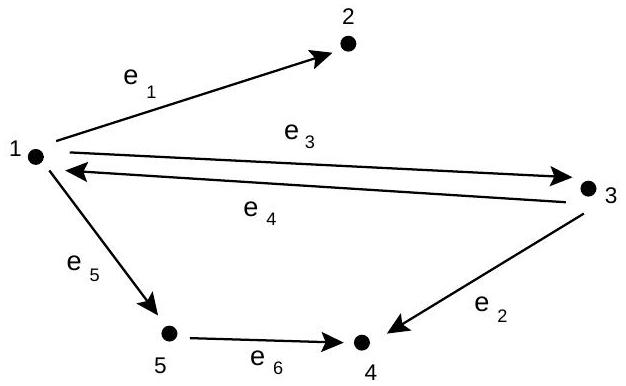
\includegraphics[max width=\textwidth, center]{2025_09_05_93c7c1835f249f70c0eeg-02}

Este es un grafo dirigido, conexo, pero no fuertemente conexo (no hay un camino dirigido de 2 a 3 ).\\
La sucesión $\left(e_{1}, e_{3}\right)$ es un camino simple de 2 a 3 . Este camino no es dirigido. El grafo no es acíclico: la sucesión ( $e_{5}, e_{6}, e_{2}, e_{3}$ ) es un ciclo. Este ciclo no es un ciclo dirigido.\\
La sucesión $\left(e_{4}, e_{5}, e_{6}\right)$ es un camino dirigido simple de 3 a 4 . La sucesión $\left(e_{3}, e_{4}\right)$ es un ciclo dirigido. La sucesión $\left(e_{1}, e_{4}, e_{2}, e_{6}, e_{5}\right)$ es un camino de 2 a 1 . Este camino no es dirigido ni simple.\\
El grafo no es completo: $(2,1) \notin E$.\\
Ejemplo 1.7. Consideremos el grafo no dirigido $G=(V, E)$, con vértices $1,2,3,4,5$ y 6 y ramas $e_{1}=(1,4)$, $e_{2}=(1,2), e_{3}=(2,5), e_{4}=(1,3)$ y $e_{5}=(5,6) V=\{1,2,3,4,5,6\}$ y $E=\{(1,4),(1,2),(2,5),(1,3),(5,6)\}$, al que representaremos gráficamente en la forma\\
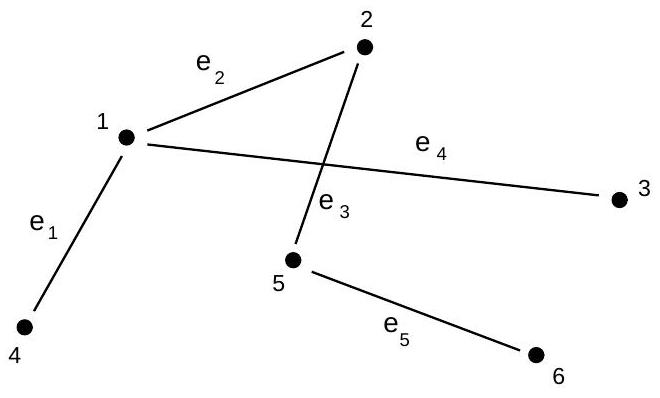
\includegraphics[max width=\textwidth, center]{2025_09_05_93c7c1835f249f70c0eeg-02(3)}

Este es un grafo no dirigido, conexo y acíclico. No es completo: $(4,5) \notin E$. La sucesión $\left(e_{1}, e_{2}, e_{3}, e_{5}\right)$ es un camino simple de 4 a 6 .

Ejemplo 1.8. Consideremos el grafo\\
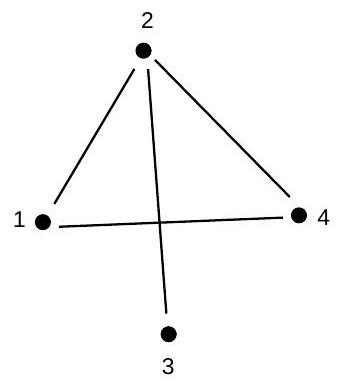
\includegraphics[max width=\textwidth, center]{2025_09_05_93c7c1835f249f70c0eeg-02(1)}\\
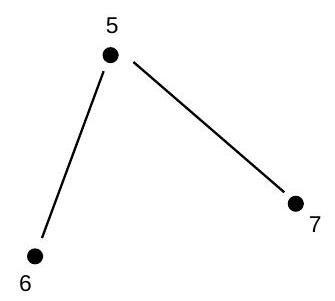
\includegraphics[max width=\textwidth, center]{2025_09_05_93c7c1835f249f70c0eeg-02(2)}

Este es un grafo no dirigido. No es conexo (no existe ningún camino que una 1 y 7 ) sino que tiene dos componentes conexas, una conteniendo un ciclo (el ciclo $(1,2),(2,4),(4,1)$ ) y otra acíclica.

Definición 1.9 Diremos que $G=(V, E)$ es un grafo bipartito si existen dos conjuntos disjuntos $P$ y $Q$ tales que $V=P \cup Q$ y toda rama $e \in E$ tiene un extremo en $P$ y el otro extremo en $Q$.

Ejemplo 1.10. El grafo\\
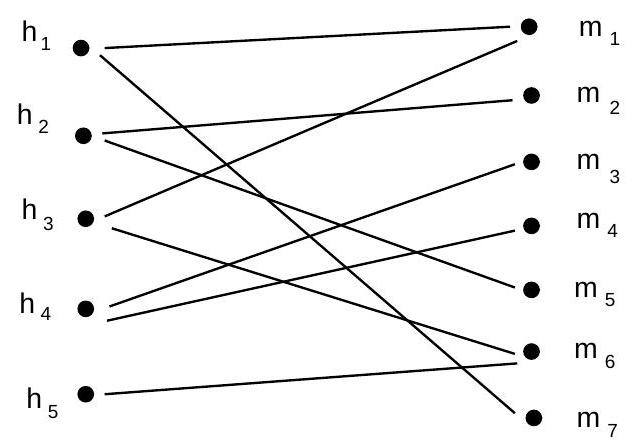
\includegraphics[max width=\textwidth, center]{2025_09_05_93c7c1835f249f70c0eeg-03(1)}\\
es bipartito. En este caso $P=\left\{h_{1}, h_{2}, h_{3}, h_{4}, h_{5}\right\}$ y $Q=\left\{m_{1}, m_{2}, m_{3}, m_{4}, m_{5}, m_{6}, m_{7}\right\}$.\\
Definición 1.11. Sea $G=(V, E)$ un grafo dirigido. Si $(u, v) \in E$ diremos que $u$ es la cola y que $v$ es la punta de la flecha ( $u, v$ ).

A cada grafo dirigido $G=(V, E)$ le podemos asociar una matriz que contiene toda la información sobre el grafo. Esta matriz se llama la matriz de incidencia vértice-rama de G .\\
Si $V=\left\{v_{1}, \ldots, v_{m}\right\}$ y $E=\left\{e_{1}, \ldots, e_{n}\right\}$, la matriz de incidencia vértice-rama de $G$ es la matriz $\left\|a_{i j}\right\| \in \mathbb{R}^{m \times n}$, definida por

$$
a_{i j}= \begin{cases}1 & \text { si } v_{i} \text { es la cola de } e_{j} \\ -1 & \text { si } v_{i} \text { es la punta de } e_{j} \\ 0 & \text { en otro caso }\end{cases}
$$

Ejemplo 1.12. Dado el grafo\\
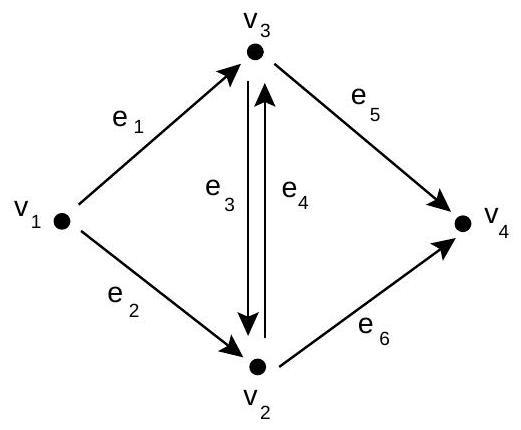
\includegraphics[max width=\textwidth, center]{2025_09_05_93c7c1835f249f70c0eeg-03}\\
su matriz de incidencia vértice-rama es la matriz

$$
A=\left(\begin{array}{cccccc}
1 & 1 & 0 & 0 & 0 & 0 \\
0 & -1 & -1 & 1 & 0 & 1 \\
-1 & 0 & 1 & -1 & 1 & 0 \\
0 & 0 & 0 & 0 & -1 & -1
\end{array}\right)
$$

Observación 1.13. La matriz de incidencia vértice-rama de un grafo $G$ tiene, en cada columna, un 1 , un -1 y el resto de los coeficientes nulos. Esto se debe a que cada rama tiene una sola cola y una sola punta. Luego, en una matriz de incidencia vértice-rama la suma de todas las filas es cero.

\section*{2. Forestas, árboles y hojas.}
Definición 2.1. Una foresta es un grafo acíclico. Un árbol es un grafo acíclico conexo, es decir, una componente conexa de una foresta.

Definición 2.2. Sea $G=(V, E)$ un grafo y sea $u \in V$. Definimos

$$
\begin{array}{ll}
i(u)=\#\{v \in V /(v, u) \in E\} & \text { indegree de } u \\
o(u)=\#\{v \in V /(u, v) \in E\} & \text { outdegree de } u
\end{array}
$$

y definimos el grado de $u$ como

$$
\operatorname{deg}(u)= \begin{cases}i(u)+o(u) & \text { si } G \text { es dirigido } \\ i(u) & \text { si } G \text { es no dirigido }\end{cases}
$$

Tanto en el caso dirigido como no dirigido resulta que $\operatorname{deg}(u)$ es el número de ramas que inciden en el vértice $u$. (Observemos que si $G$ es no dirigido entonces los conjuntos que definen $i(u)$ y $o(u)$ son iguales y por eso no los contamos dos veces).

Definición 2.3. Sea $G=(V, E)$ un árbol. Diremos que $u \in V$ es una hoja sii deg $(u) \leq 1$, es decir, una hoja es un vértice en el que incide a lo sumo una rama.

Observación 2.4. Si $G$ es un árbol con un único vértice (y ninguna rama) entonces ese vértice es una hoja. En cualquier otro caso, un árbol siempre tiene por lo menos dos hojas.

Ejemplo 2.5. El grafo no dirigido\\
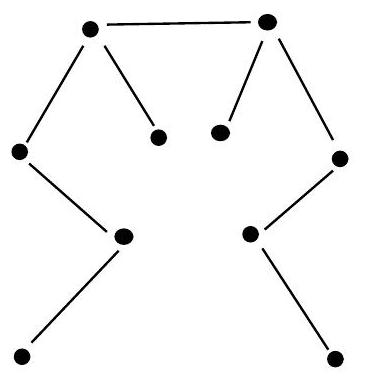
\includegraphics[max width=\textwidth, center]{2025_09_05_93c7c1835f249f70c0eeg-04(2)}\\
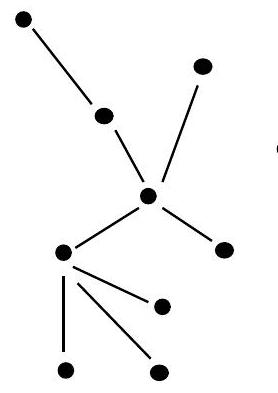
\includegraphics[max width=\textwidth, center]{2025_09_05_93c7c1835f249f70c0eeg-04}\\
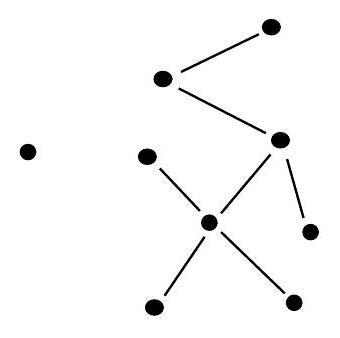
\includegraphics[max width=\textwidth, center]{2025_09_05_93c7c1835f249f70c0eeg-04(1)}\\
es una foresta compuesta por cuatro árboles. El primero tiene cuatro hojas, el segundo seis, el tercero una y el cuarto cinco.

Ejemplo 2.6. El grafo dirigido\\
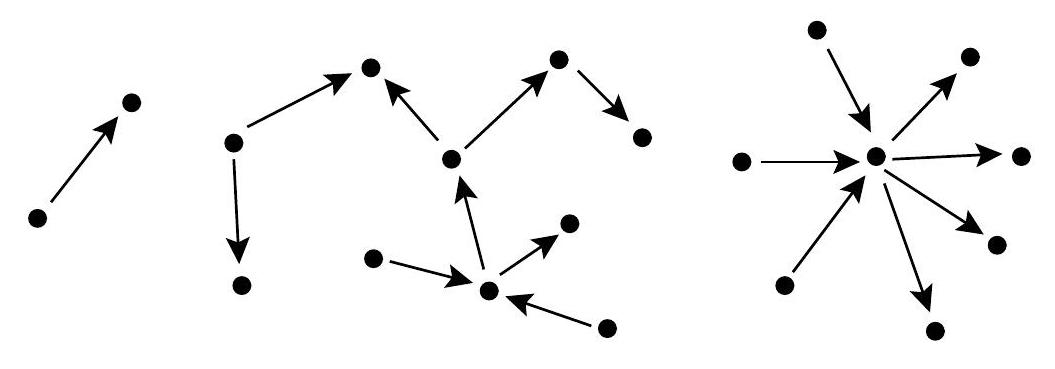
\includegraphics[max width=\textwidth, center]{2025_09_05_93c7c1835f249f70c0eeg-04(3)}\\
es una foresta compuesta por tres árboles con dos, cinco y siete hojas cada uno respectivamente.\\
Definición 2.7. Un árbol binario es un árbol dirigido $G=(V, E)$ tal que $o(u)=2$ para todo $u \in V$ que no sea una hoja.

Ejemplo 2.8. El grafo dirigido\\
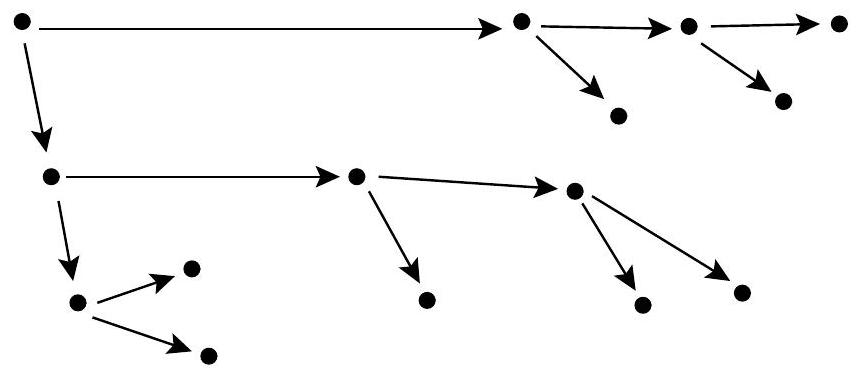
\includegraphics[max width=\textwidth, center]{2025_09_05_93c7c1835f249f70c0eeg-05}\\
es un árbol binario. También lo es el grafo\\
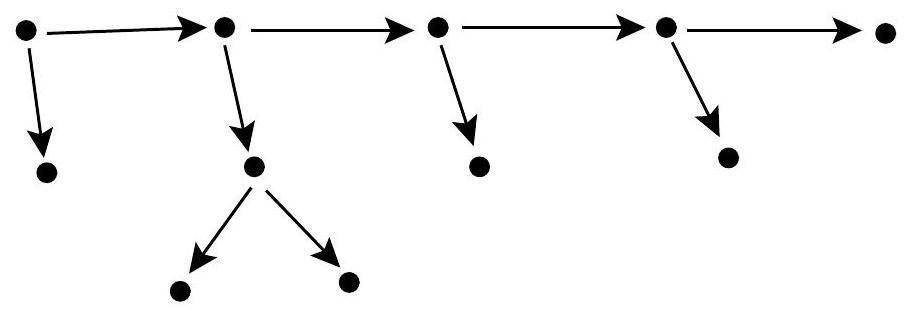
\includegraphics[max width=\textwidth, center]{2025_09_05_93c7c1835f249f70c0eeg-05(1)}

Proposición 2.9. Si un árbol tiene $n$ ramas entonces tiene $n+1$ vértices.\\
Demostración: Por inducción en $n$.\\
El caso $n=1$ es trivial. Supongamos que la proposición vale para todo árbol con $n$ ramas y sea $G$ un árbol con $n+1$ ramas. Sea $u$ una hoja de $G$ y sea $e$ la única rama de $G$ que incide en $u$ (es decir, $e=(w, u) \in E$ si $i(u)=1$ y $\{v \in V /(v, u) \in E\}=\{(w, u)\}$ o bien $e=(u, w) \in E$ si $o(u)=1$ y $\{v \in V /(u, v) \in E\}=\{(u, w)\}$. Sea $G^{\prime}=\left(V^{\prime}, E^{\prime}\right)$, donde $V^{\prime}=V-\{u\}$ y $E^{\prime}=E-\{e\}$. Entonces $G^{\prime}$ es un árbol con $n$ ramas. Luego, por hipótesis inductiva, $\# V^{\prime}=n+1$, de donde $\# V=n+2$. ㅁ

Proposición 2.10. Si $G$ es un grafo conexo con $m$ vértices y $m-1$ ramas entonces $G$ es un árbol.\\
Demostración: Sólo debemos ver que $G$ es acíclico.\\
Supongamos que $G$ tuviera un ciclo. Entonces, como se ve en el dibujo, podríamos quitar una rama $e_{1}$ del ciclo de manera que $G^{\prime}=\left(V, E-\left\{e_{1}\right\}\right)$ siguiera siendo conexo y tuviera un ciclo menos que $G$.\\
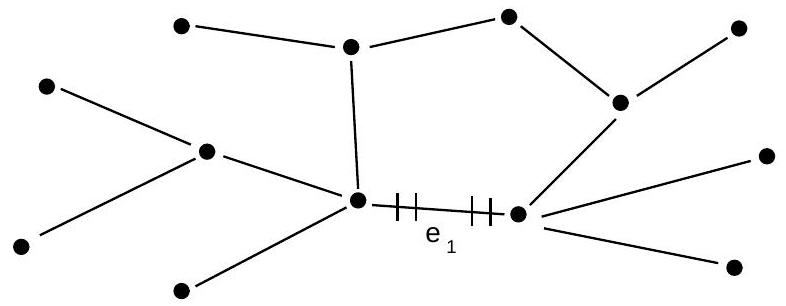
\includegraphics[max width=\textwidth, center]{2025_09_05_93c7c1835f249f70c0eeg-05(2)}

Si $G^{\prime}$ no fuera acíclico podríamos repetir el procedimiento. Así siguiendo, luego de quitar $r$ ramas obtenemos un grafo conexo y acíclico ( $V, E-\left\{e_{1}, \ldots, e_{r}\right\}$ ). Pero este árbol tendría $m$ vértices y $m-1-r<m-1$ ramas. Absurdo, pues esto contradice la proposición 2.9.

\section*{3. Grafos planares.}
Definición 3.1. Un grafo no dirigido $G$ se dice planar si se lo puede representar en el plano de manera tal que sus ramas sólo se corten en los vértices.

Ejemplo 3.2. El grafo\\
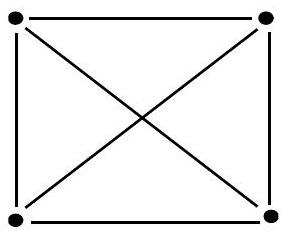
\includegraphics[max width=\textwidth, center]{2025_09_05_93c7c1835f249f70c0eeg-06(4)}\\
es planar ya que se puede representar en la forma\\
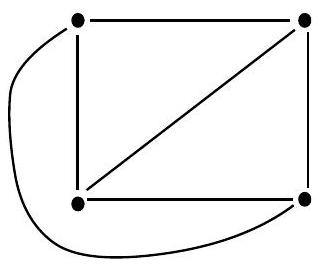
\includegraphics[max width=\textwidth, center]{2025_09_05_93c7c1835f249f70c0eeg-06}

Ejemplo 3.3. No son planares\\
i) el grafo bipartito completo $K_{3,3}$ de $3 \times 3$\\
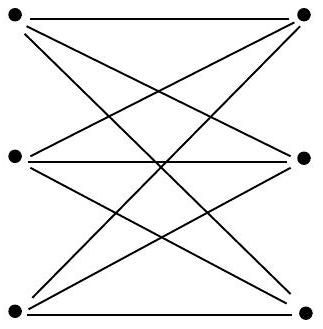
\includegraphics[max width=\textwidth, center]{2025_09_05_93c7c1835f249f70c0eeg-06(3)}\\
ii) el grafo completo $K_{5}$ de cinco vértices\\
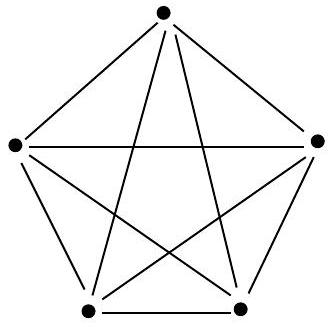
\includegraphics[max width=\textwidth, center]{2025_09_05_93c7c1835f249f70c0eeg-06(2)}

Un grafo planar divide al plano en regiones conexas a las que llamaremos caras. Dado un grafo planar, siempre una de sus caras es no acotada.

Ejemplo 3.4. El grafo\\
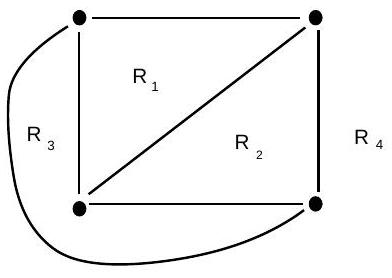
\includegraphics[max width=\textwidth, center]{2025_09_05_93c7c1835f249f70c0eeg-06(1)}\\
divide al plano en cuatro regiones $R_{1}, \ldots, R_{4}$. La cara $R_{4}$ no es acotada.

Ejemplo 3.5. El grafo\\
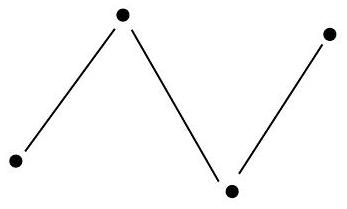
\includegraphics[max width=\textwidth, center]{2025_09_05_93c7c1835f249f70c0eeg-07}\\
tiene una sola cara.\\
Un resultado clásico sobre el número de caras, vértices y ramas de un grafo es el siguiente.\\
Teorema 3.6. (Euler) Sean $V, E$ y $F$ los conjuntos de vértices, ramas y caras de un grafo planar conexo. Entonces $\# V-\# E+\# F=2$.\\
Demostración: Por inducción en $\# F$. Si $\# F=1$ tenemos un grafo conexo con una sola cara, es decir, un árbol. En este caso, $\# E=\# V-1$. Luego $\# V-\# E+1=2$ como queríamos ver.\\
Supongamos ahora que $\# F=n+1$ y que el teorema vale para todo grafo con $n$ caras. Sea $e$ una rama que separa dos caras. Entonces el grafo que resulta de quitar esa rama es un grafo planar conexo que tiene una cara menos, la misma cantidad de vértices y una rama menos. Entonces, por hipótesis inductiva $\# V-(\# E-1)+(\# F-1)=2$. Por lo tanto $\# V-\# E+\# F=2$. ㅁ

Recordemos que si un grafo $G=(V, E)$ es completo y $m=\# V$ entonces

$$
\# E= \begin{cases}\binom{m}{2}=\frac{m(m-1)}{2} & \text { si } G \text { es no dirigido } \\ \binom{m}{2} .2!=m(m-1) & \text { si } G \text { es dirigido }\end{cases}
$$

En cambio, en un grafo planar las ramas son relativamente escasas como lo muestra la siguiente proposición.\\
Proposición 3.7. Un grafo planar conexo con $m \geq 3$ vértices tiene a lo sumo $3(\mathrm{~m}-2)$ ramas.\\
Demostración: Cada cara del grafo está delimitada por un circuito que tiene por lo menos tres ramas (salvo el caso $\# E=2$ en cuyo caso debe ser $m=3$ y vale trivialmente lo que queremos probar).\\
Para cada cara $R_{i}$ sea $x_{i}$ la cantidad de ramas que son un borde de $R_{i}$. Entonces

$$
\sum_{i=1}^{\# F} x_{i} \geq 3 \# F
$$

Por otra parte, como cada rama es el borde de a lo sumo dos caras entonces

$$
\sum_{i=1}^{\# F} x_{i} \leq 2 \# E
$$

Luego, $2 \# E \geq 3 \# F$. Ahora, aplicando el teorema 3.6. de Euler, se tiene que

$$
2 \# E \geq 3(2+\# E-\# V)=6+3 \# E-3 \# V
$$

de donde $\# E \leq 3 \# V-6=3(\# V-2)=3(m-2)$ como habíamos afirmado. ㅁ

\section*{4. Buscando un camino.}
Dado un grafo $G=(V, E)$ y dado un vértice $s$ de $G$, vamos a describir un algoritmo que, para cada $t \in V$ tal que $t \neq s$, encuentra (cuando existe) un camino en $G$ de $s$ a $t$. Describiremos dos maneras de hacer esto,\\
llamadas breadth-first search y depth-first search. Para poder aplicar estos algoritmos necesitaremos conocer cierta información sobre el grafo dada en lo que llamaremos la tabla de adyacencia de $G$.

Definición 4.1. Sea $G=(V, E)$ un grafo. Dados $u, v \in V$ diremos que $u$ y $v$ son adyacentes si $(u, v) \in E$ o $(v, u) \in E$.

Dado un grafo $G=(V, E)$, la tabla de adyacencia de $G$ es una tabla que contiene, para cada vértice $u$, el conjunto $A(u)=\{v \in V / u$ y $v$ son adyacentes $\}$.

Ejemplo 4.2. La tabla de adyacencia del grafo\\
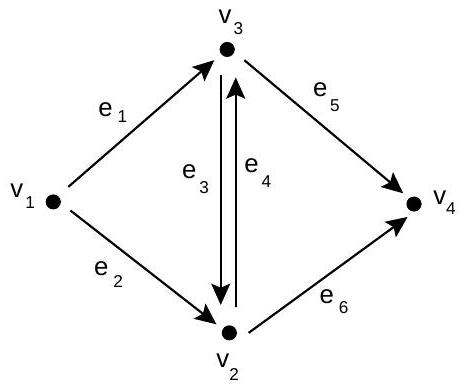
\includegraphics[max width=\textwidth, center]{2025_09_05_93c7c1835f249f70c0eeg-08}\\
es la tabla

\begin{center}
\begin{tabular}{|l|l|}
\hline
$u$ & $A(u)$ \\
\hline
$v_{1}$ & $v_{3}, v_{2}$ \\
\hline
$v_{2}$ & $v_{1}, v_{3}, v_{4}$ \\
\hline
$v_{3}$ & $v_{1}, v_{2}, v_{4}$ \\
\hline
$v_{4}$ & $v_{2}, v_{3}$ \\
\hline
\end{tabular}
\end{center}

\section*{Descripción del algoritmo breadth-first search.}
\begin{enumerate}
  \item Hacer una lista de los elementos de $V$.
  \item Marcar $s$ en la lista, poner $Q=\{s\}$ y $p(u)=-1$ para cada $u \in V$.
  \item Si $u \in Q$ es, de todos los elementos el primero que ingresó a $Q, Q=Q-\{u\}$.
  \item Para cada $v \in A(u)$ que no esté marcado en la lista, marcarlo y reemplazar $Q$ por $Q \cup\{v\}$ y $p(v)$ por $u$. Llevar un registro del orden en que los elementos ingresan a $Q$.
  \item Si $Q=\emptyset$ STOP.
  \item goto 3 .
\end{enumerate}

Al terminar el algoritmo se tiene un subconjunto de vértices que están marcados. Dado $t \neq s$ se verifica que existe un camino de $s$ a $t$ si y sólo si $t$ está marcado y en tal caso, $p(t)$ es el nodo anteriror a $t$ en ese camino. De esta manera, el camino a $t$ hallado por el algoritmo puede reconstruírse usando el predecesor $p(v)$ de cada nodo $v$ de ese camino.\\
El criterio usado para extraer cada vértice $u$ de $Q$ en este algoritmo es "first in, first out". En este caso decimos que $Q$ es una cola (queue) y la búsqueda se denomina breadth-first search. Si, en cambio, utilizamos el criterio "last in, first out" para extraer los elementos de $Q$ entonces la búsqueda se llama depth-first search y $Q$ se dice una pila (stack). Es decir, el algoritmo depth-first search resulta de cambiar en el algoritmo anterior el paso 3. por\\
3'. Si $u \in Q$ es, de todos los elementos de el último que ingresó a $Q, Q=Q-\{u\}$.\\
Observación 4.3. El grafo $G$ puede ser dirigido o no dirigido. Si el grafo es dirigido el camino no necesariamente es dirigido. Si quisiéramos resolver el problema de determinar (cuando existe) un camino dirigido\\
de $s$ a $t$ deberemos utilizar, en lugar de la tabla de adyacencia, una tabla que contenga, para cada vértice $u$, el conjunto

$$
A^{\prime}(u)=\{v \in V /(u, v) \in E\}
$$

Dejamos a cargo del lector verificar que, en ambos casos, los caminos hallados por el algoritmo search son simples.\\
A continuación aplicaremos estos algoritmos en un par de ejemplos. En el primer caso aplicaremos el algoritmo breadth-first search a un grafo no dirigido y usaremos la tabla de adyacencia del grafo para encontrar, fijado un vértice $s$, un camino de $s$ a $t$, para aquellos $t$ tales que existe un tal camino. En el segundo, aplicaremos el algoritmo depth-first search a un grafo dirigido y encontraremos, para un determinado $s$, un camino dirigido de $s$ a $t$, para aquellos $t$ tales que existe un tal camino. En este caso usaremos, en lugar de la tabla de adyacencia, la tabla que contiene, para cada $u$, el conjunto $A^{\prime}(u)$.

Ejemplo 4.4. Dado el grafo\\
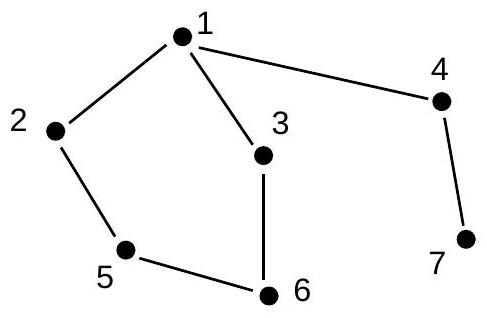
\includegraphics[max width=\textwidth, center]{2025_09_05_93c7c1835f249f70c0eeg-09}\\
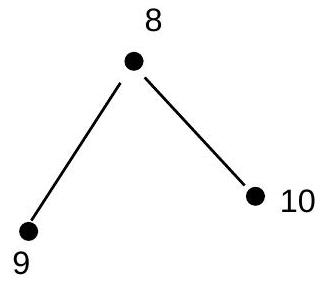
\includegraphics[max width=\textwidth, center]{2025_09_05_93c7c1835f249f70c0eeg-09(1)}\\
su tabla de adyacencia es

\begin{center}
\begin{tabular}{|c|l|}
\hline
$u$ & $A(u)$ \\
\hline
1 & $2,3,4$ \\
\hline
2 & 1,5 \\
\hline
3 & 1,6 \\
\hline
4 & 1,7 \\
\hline
5 & 2,6 \\
\hline
6 & 3,5 \\
\hline
7 & 4 \\
\hline
8 & 9,10 \\
\hline
9 & 8 \\
\hline
10 & 8 \\
\hline
\end{tabular}
\end{center}

Sea $s=1$. Determinaremos, usando breadth-first search, para cuáles $t$ existe un camino de $s$ a $t$. Reconstruiremos ese camino para uno de esos valores de $t$ y dejaremos a cargo del lector la reconstrucción de los caminos a los restantes $t$ hallados.

\begin{enumerate}
  \item $V=\{1,2,3,4,5,6,7,8,9,10\}$
  \item $V=\left\{1^{*}, 2,3,4,5,6,7,8,9,10\right\}, Q=\{1\}, p=(p(1), p(2), \ldots, p(10))=(-1,-1, \ldots,-1)$
\end{enumerate}

Primera iteración\\
3. $u=1, Q=Q-\{1\}=\emptyset$\\
4. $A(u)=\{2,3,4\}$, marcamos 2,3 y 4 , los agregamos a la cola y reemplazamos $p(2), p(3)$ y $p(4)$ por 1 . El estado actual de la lista y de la cola es\\
$V=\left\{1^{*}, 2^{*}, 3^{*}, 4^{*}, 5,6,7,8,9,10\right\}$ y $Q=\{2,3,4\}$.\\
El valor actual del vector $p$ es $(-1,1,1,1,-1,-1,-1,-1,-1,-1)$\\
5. $Q \neq \emptyset$\\
6. volvemos a 3 .

Segunda iteración\\
3. $u=2, Q=Q-\{2\}=\{3,4\}$\\
4. $A(u)=\{1,5\}$, marcamos el 5 , lo agregamos a la cola y reemplazamos $p(5)$ por 2 . El estado actual de la lista y de la cola es $V=\left\{1^{*}, 2^{*}, 3^{*}, 4^{*}, 5^{*}, 6,7,8,9,10\right\}$ y $Q=\{3,4,5\}$.\\
El valor actual del vector $p$ es $(-1,1,1,1,2,-1,-1,-1,-1,-1)$\\
5. $Q \neq \emptyset$\\
6. volvemos a 3 .

Tercera iteración\\
3. $u=3, Q=Q-\{3\}=\{4,5\}$\\
4. $A(u)=\{1,6\}$, marcamos el 6 , lo agregamos a la cola y reemplazamos $p(6)$ por 3 . El estado actual de la lista y de la cola es $V=\left\{1^{*}, 2^{*}, 3^{*}, 4^{*}, 5^{*}, 6^{*}, 7,8,9,10\right\}$ y $Q=\{4,5,6\}$.\\
El valor actual del vector $p$ es $(-1,1,1,1,2,3,-1,-1,-1,-1)$\\
5. $Q \neq \emptyset$

6 . volvemos a 3 .\\
Cuarta iteración\\
3. $u=4, Q=Q-\{4\}=\{5,6\}$\\
4. $A(u)=\{1,7\}$, marcamos el 7 , lo agregamos a la cola y reemplazamos $p(7)$ por 4 . El estado actual de la lista y de la cola es\\
$V=\left\{1^{*}, 2^{*}, 3^{*}, 4^{*}, 5^{*}, 6^{*}, 7^{*}, 8,9,10\right\}$ y $Q=\{5,6,7\}$.\\
El valor actual del vector $p$ es $(-1,1,1,1,2,3,4,-1,-1,-1)$\\
5. $Q \neq \emptyset$

6 . volvemos a 3 .\\
Quinta iteración\\
3. $u=5, Q=Q-\{5\}=\{6,7\}$\\
4. $A(u)=\{2,6\}$, no marcamos ningún vértice porque el 2 y el 6 ya están marcados. El estado actual de la lista y de la cola es\\
$V=\left\{1^{*}, 2^{*}, 3^{*}, 4^{*}, 5^{*}, 6^{*}, 7^{*}, 8,9,10\right\}$ y $Q=\{6,7\}$.\\
El valor actual del vector $p$ es $(-1,1,1,1,2,3,4,-1,-1,-1)$\\
5. $Q \neq \emptyset$

6 . volvemos a 3 .\\
Sexta iteración\\
3. $u=6, Q=Q-\{6\}=\{7\}$\\
4. $A(u)=\{3,5\}$, no marcamos ningún vértice porque el 3 y el 5 ya están marcados. El estado actual de la lista y de la cola es\\
$V=\left\{1^{*}, 2^{*}, 3^{*}, 4^{*}, 5^{*}, 6^{*}, 7^{*}, 8,9,10\right\}$ y $Q=\{7\}$.\\
El valor actual del vector $p$ es $(-1,1,1,1,2,3,4,-1,-1,-1)$\\
5. $Q \neq \emptyset$

6 . volvemos a 3 .\\
Séptima iteración\\
3. $u=7, Q=Q-\{7\}=\emptyset$\\
4. $A(u)=\{4\}$, no marcamos ningún vértice porque el 4 ya está marcado. El estado actual de la lista y de la cola es\\
$V=\left\{1^{*}, 2^{*}, 3^{*}, 4^{*}, 5^{*}, 6^{*}, 7^{*}, 8,9,10\right\}$ y $Q=\emptyset$.

El valor actual del vector $p$ es ( $-1,1,1,1,2,3,4,-1,-1,-1$ )\\
5. $Q=\emptyset$. STOP

Dado $t \neq 1$, existe un camino de 1 a $t$ sii $t=2,3,4,5,6,7$.\\
Como $p(6)=3$ y $p(3)=1$ entonces el camino de $s=1$ a $t=6$ hallado por el algoritmo es\\
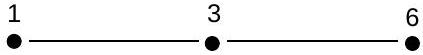
\includegraphics[max width=\textwidth, center]{2025_09_05_93c7c1835f249f70c0eeg-11(1)}

Dejamos a cargo del lector la reconstrucción de los caminos a los restantes $t$ hallados.\\
Ejemplo 4.5. Dado el grafo dirigido\\
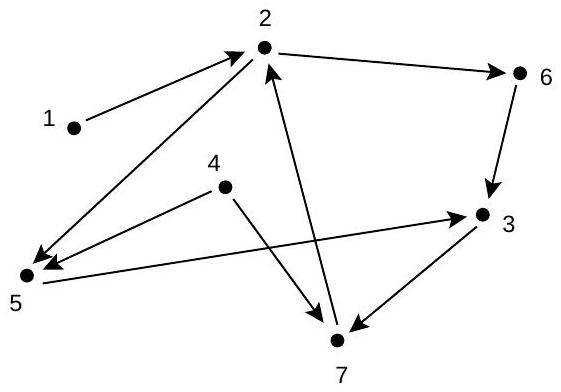
\includegraphics[max width=\textwidth, center]{2025_09_05_93c7c1835f249f70c0eeg-11}\\
construyamos la tabla

\begin{center}
\begin{tabular}{|l|l|}
\hline
$u$ & $A^{\prime}(u)$ \\
\hline
1 & 2 \\
\hline
2 & 5,6 \\
\hline
3 & 7 \\
\hline
4 & 5,7 \\
\hline
5 & 3 \\
\hline
6 & 3 \\
\hline
7 & 2 \\
\hline
\end{tabular}
\end{center}

Sea $s=1$. Determinaremos, usando depdth-first search, para cuáles $t$ existe un camino dirigido de $s$ a $t$. Reconstruiremos ese camino para uno de esos valores de $t$ y dejaremos a cargo del lector la reconstrucción de los caminos a los restantes $t$ hallados.

\begin{enumerate}
  \item $V=\{1,2,3,4,5,6,7\}$
  \item $V=\left\{1^{*}, 2,3,4,5,6,7\right\}, Q=\{1\}, p=(p(1), p(2), \ldots, p(7))=(-1,-1, \ldots,-1)$
\end{enumerate}

Primera iteración\\
3. $u=1, Q=Q-\{1\}=\emptyset$\\
4. $A^{\prime}(u)=\{2\}$, marcamos 2 , lo ponemos en la pila y reemplazamos $p(2)$ por 1 . El estado actual de la lista y de la pila es\\
$V=\left\{1^{*}, 2^{*}, 3,4,5,6,7\right\}$ y $Q=\{2\}$.\\
El valor actual del vector $p$ es $(-1,1,-1,-1,-1,-1,-1)$\\
5. $Q \neq \emptyset$\\
6. volvemos a 3 .

Segunda iteración\\
3. $u=2, Q=Q-\{2\}=\emptyset$\\
4. $A^{\prime}(u)=\{5,6\}$, marcamos 5,6 , los ponemos en la pila y reemplazamos $p(5)$ y $p(6)$ por 2 . El estado actual de la lista y de la pila es\\
$V=\left\{1^{*}, 2^{*}, 3,4,5^{*}, 6^{*}, 7\right\}$ y $Q=\{5,6\}$

El valor actual del vector $p$ es $(-1,1,-1,-1,2,2,-1)$\\
5. $Q \neq \emptyset$\\
6. volvemos a 3 .

Tercera iteración\\
3. $u=6, Q=Q-\{6\}=\{5\}$\\
4. $A^{\prime}(u)=\{3\}$, marcamos el 3 , lo ponemos en la pila y reemplazamos $p(3)$ por 6 . El estado actual de la lista y de la pila es\\
$V=\left\{1^{*}, 2^{*}, 3^{*}, 4,5^{*}, 6^{*}, 7\right\}$ y $Q=\{5,3\}$\\
El valor actual del vector $p$ es $(-1,1,6,-1,2,2,-1)$\\
5. $Q \neq \emptyset$\\
6. volvemos a 3 .

Cuarta iteración\\
3. $u=3, Q=Q-\{3\}=\{5\}$\\
4. $A^{\prime}(u)=\{7\}$, marcamos 7, lo ponemos en la pila y reemplazamos $p(7)$ por 3 . El estado actual de la lista y de la pila es\\
$V=\left\{1^{*}, 2^{*}, 3^{*}, 4,5^{*}, 6^{*}, 7^{*}\right\}$ y $Q=\{5,7\}$\\
El valor actual del vector $p$ es $(-1,1,6,-1,2,2,3)$\\
5. $Q \neq \emptyset$\\
6. volvemos a 3 .

Quinta iteración\\
3. $u=7, Q=Q-\{7\}=\{5\}$\\
4. $A^{\prime}(u)=\{2\}$, no marcamos ningún vértice porque 2 ya está marcado. El estado actual de la lista y de la pila es\\
$V=\left\{1^{*}, 2^{*}, 3^{*}, 4,5^{*}, 6^{*}, 7^{*}\right\}$ y $Q=\{5\}$\\
El valor actual del vector $p$ es $(-1,1,6,-1,2,2,3)$.\\
5. $Q \neq \emptyset$\\
6. volvemos a 3 .

Sexta iteración\\
3. $u=5, Q=Q-\{5\}=\emptyset$\\
4. $A^{\prime}(u)=\{3\}$, no marcamos ningún vértice porque 3 ya está marcado. El estado actual de la lista y de la pila es\\
$V=\left\{1^{*}, 2^{*}, 3^{*}, 4,5^{*}, 6^{*}, 7^{*}\right\}$ y $Q=\emptyset$\\
El valor actual del vector $p$ es $(-1,1,6,-1,2,2,3)$.\\
5. $Q=\emptyset$. STOP.

Dado $t \neq 1$, existe un camino dirigido de 1 a $t$ sii $t=2,3,5,6,7$.\\
Como $p(7)=3, p(3)=6, p(6)=2$ y $p(2)=1$ entonces el camino de $s=1$ a $t=7$ hallado por el algoritmo es $1 \longrightarrow 2 \longrightarrow 6 \longrightarrow 3 \longrightarrow 7$.\\
Como antes, dejamos a cargo del lector la reconstrucción de los caminos a los restantes $t$ hallados.

\section*{Complejidad del algoritmo.}
Estimaremos ahora la complejidad del algoritmo search, es decir, la cantidad de operaciones que realiza el algoritmo para obtener el output a partir de los datos de entrada.\\
Sea $m=\# V$. El algoritmo realiza a lo sumo $m$ iteraciones (pues cada vértice ingresa en $Q$ a lo sumo una vez: al ingresar un vértice, se lo marca y los vértices que están marcados no se ingresan) y, en cada una de ellas, se realizan a lo sumo $c m$ operaciones, para una constante $c>0$. Luego, el algoritmo realiza en total a\\
lo sumo $c m^{2}$ operaciones y por lo tanto la complejidad del algoritmo search es menor o igual que $c m^{2}$ para una constante $c$. Diremeos entonces que la complejidad es del orden de $m^{2}$ o también que es $O\left(m^{2}\right)$.\\
Definición 4.5. Dado un algoritmo, sea $N$ el tamaño del input, es decir, la cantidad de bits que se necesitan para describir el input. Diremos que la complejidad del algoritmo es polinomial si es menor o igual que $P(N)$ para algún polinomio $P$.\\
En el caso del algoritmo search, se tiene que $m \leq N$, de donde $c m^{2} \leq c . N^{2}$. Luego, la complejidad del algoritmo search es menor o igual que $P(N)$ donde $P$ es el polinomio $c X^{2}$. Hemos probado entonces que la complejidad de este algorimto es polinomial.

\section*{5. Spanning trees.}
Definición 5.1. Sea $G=(V, E)$ un grafo conexo. Un spanning tree de $G$ es un árbol $T=\left(V^{\prime}, E^{\prime}\right)$ tal que $V^{\prime}=V$ y $E^{\prime}$ es un subconjunto de $E$.

Ejemplo 5.2. Si $G$ es el grafo\\
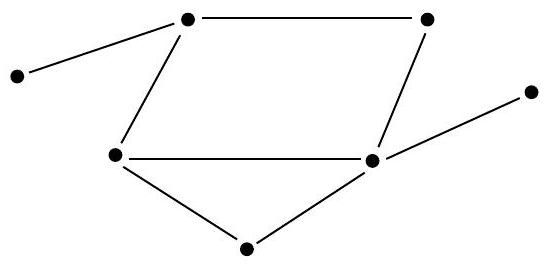
\includegraphics[max width=\textwidth, center]{2025_09_05_93c7c1835f249f70c0eeg-13}\\
entonces el grafo\\
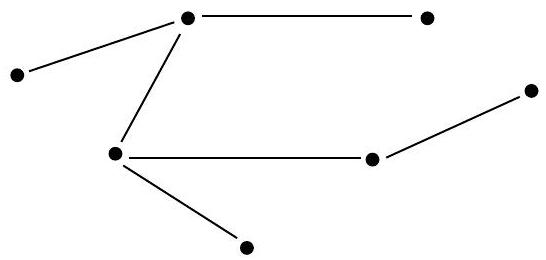
\includegraphics[max width=\textwidth, center]{2025_09_05_93c7c1835f249f70c0eeg-13(1)}\\
es un spanning tree de $G$. También lo es el grafo\\
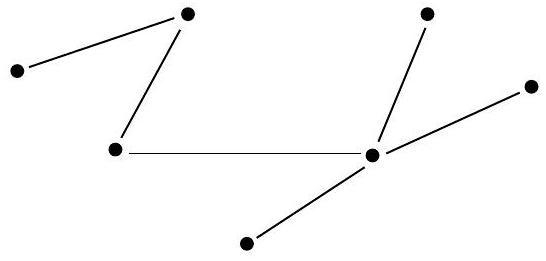
\includegraphics[max width=\textwidth, center]{2025_09_05_93c7c1835f249f70c0eeg-13(2)}

Observación 5.3. Sea $G$ un grafo conexo. Si $G$ es un árbol, entonces $G$ es un spanning tree de $G$ y es el único posible. Pero si $G$ no es un árbol, entonces contiene por lo menos un ciclo. Siguiendo la misma idea que en la proposición 2.10., podemos quitar una rama del ciclo de manera que el subgrafo resultante siga siendo conexo y tenga un ciclo menos. Si este no es un grafo acíclico, repetimos el procedimiento. De esta manera luego de un número finito de pasos obtenemos un subgrafo conexo acíclico de $G$. Como este grafo fue obtenido quitando sólo ramas y no vértices, entonces es un spanning tree de $G$. Esto muestra que cualquier grafo conexo tiene un spanning tree.\\
Observación 5.4. Sea $G=(V, E)$ un grafo conexo con $m$ vértices. Si $G^{\prime}=\left(V^{\prime}, E^{\prime}\right)$ es un subgrafo conexo y acíclico de $G$ con $m-1$ ramas entonces $G^{\prime}$ es un spannig tree de $G$. En efecto, como $G^{\prime}$ es un árbol con\\
$m-1$ ramas, entonces $\# V^{\prime}=m$ por la proposición 2.9. Pero $V^{\prime} \subseteq V, \# V^{\prime}=m=\# V$ y $E^{\prime} \subseteq E$. Luego $V^{\prime}=V$ y $E^{\prime} \subseteq E$.\\
Sea $G$ un grafo no dirigido y conexo donde a cada rama $e$ de $G$ se le ha asignado un peso $\omega(e)$.\\
Definición 5.5. Diremos que un spanning tree $T$ de $G$ es mínimo sii la suma de los pesos de sus ramas es menor o igual que la suma de los pesos de las ramas de cualquier otro spanning tree de $G$.

Ejemplo 5.6. Consideremos el siguiente grafo donde en cada rama indicamos el peso\\
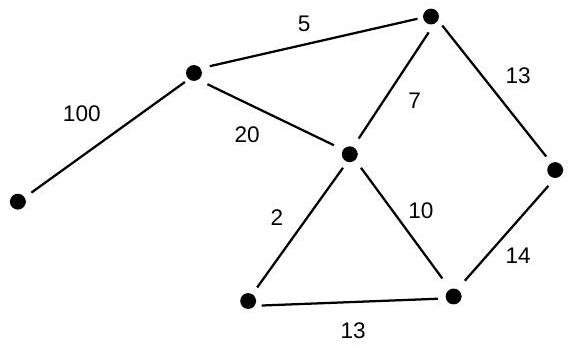
\includegraphics[max width=\textwidth, center]{2025_09_05_93c7c1835f249f70c0eeg-14(1)}

Entonces $T$ dado por\\
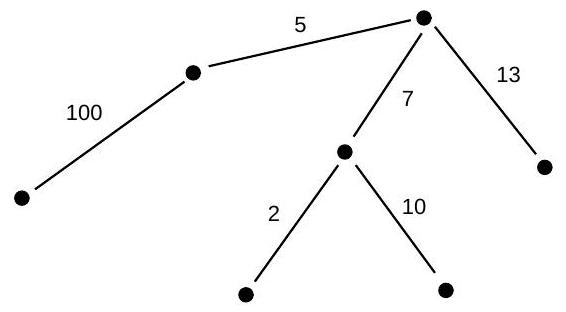
\includegraphics[max width=\textwidth, center]{2025_09_05_93c7c1835f249f70c0eeg-14(2)}\\
es un spanning tree mínimo de $G$. La suma de los pesos de sus ramas es 137 .\\
Ejemplo 5.7. Supongamos que deseamos interconectar cinco localidades con una red de caminos a costo mínimo. Supongamos conocido el costo de conectar las localidades $i$ y $j$ e ilustremos la situación con esos datos en un grafo $G$ con pesos, donde a cada rama $(i, j)$ le asignamos como peso el costo de conectar $i$ y $j$.\\
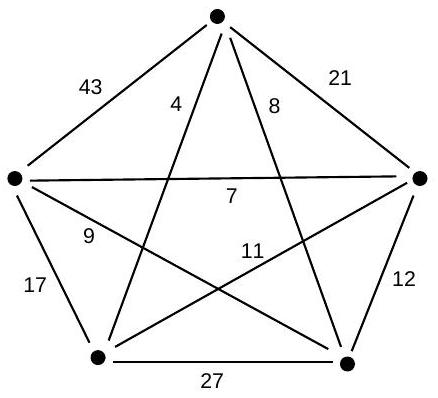
\includegraphics[max width=\textwidth, center]{2025_09_05_93c7c1835f249f70c0eeg-14}

Entonces la solución del problema consiste en hallar un spanning tree mínimo de $G$.\\
En las próximas dos secciones veremos un par de algoritmos que hallan, dado un grafo $G$ no dirigido, conexo y con pesos, un spanning tree mínimo de $G$.

\section*{6. El algoritmo de Kruskal}
Sea $G=(V, E)$ un grafo no dirigido, conexo, donde cada rama $e \in E$ tiene asignado un peso $\omega(e)$. Sea\\
$m=\# V$. El siguiente algoritmo, conocido como el algoritmo de Kruskal encuentra, en tiempo polinomial, un spanning tree mínimo de $G$.

\section*{Descripción del algoritmo.}
\begin{enumerate}
  \item Ordenar las ramas de $G$ de menor a mayor según el peso.
  \item Elegir una rama de mínimo peso entre aquellas que todavía no fueron elegidas y que no forman un ciclo con las ya elegidas.
  \item repetir 2. si el número de ramas elegidas es menor que $m-1$.
\end{enumerate}

Ejemplo 6.1. Apliquemos el algoritmo al grafo $G$ con $m=8$ vértices dado por\\
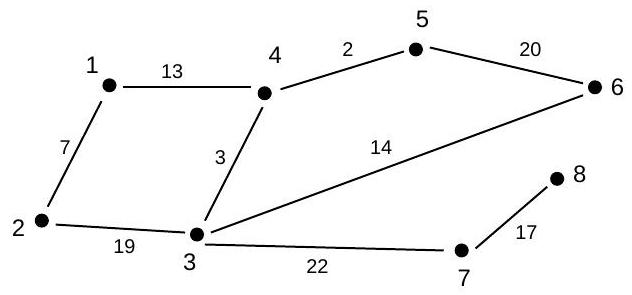
\includegraphics[max width=\textwidth, center]{2025_09_05_93c7c1835f249f70c0eeg-15(1)}

Para poder tener en claro en el gráfico cuál es el conjunto de ramas elegidas, dibujaremos las ramas que han sido elegidas hasta el momento con trazo grueso y las que no con trazo fino.

\begin{enumerate}
  \item Ordenamos las ramas de menor a mayor según el peso tal como se indica en la tabla
\end{enumerate}

\begin{center}
\begin{tabular}{|c|c|}
\hline
$e$ & $\omega(e)$ \\
\hline
$e_{1}=(4,5)$ & $\omega\left(e_{1}\right)=2$ \\
\hline
$e_{2}=(4,3)$ & $\omega\left(e_{2}\right)=3$ \\
\hline
$e_{3}=(1,2)$ & $\omega\left(e_{3}\right)=7$ \\
\hline
$e_{4}=(1,4)$ & $\omega\left(e_{4}\right)=13$ \\
\hline
$e_{5}=(3,6)$ & $\omega\left(e_{5}\right)=14$ \\
\hline
$e_{6}=(7,8)$ & $\omega\left(e_{6}\right)=17$ \\
\hline
$e_{7}=(2,3)$ & $\omega\left(e_{7}\right)=19$ \\
\hline
$e_{8}=(5,6)$ & $\omega\left(e_{8}\right)=20$ \\
\hline
$e_{9}=(3,7)$ & $\omega\left(e_{9}\right)=22$ \\
\hline
\end{tabular}
\end{center}

\begin{enumerate}
  \setcounter{enumi}{1}
  \item Elegimos $e_{1}$.\\
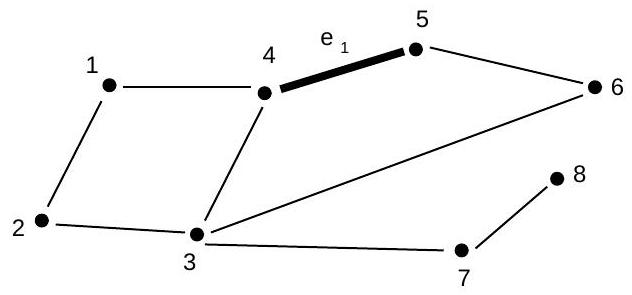
\includegraphics[max width=\textwidth, center]{2025_09_05_93c7c1835f249f70c0eeg-15}
\end{enumerate}

Como $\#\{$ ramas elegidas $\}=1<8-1=m-1$, repetimos 2. Ahora elegimos $e_{2}$.\\
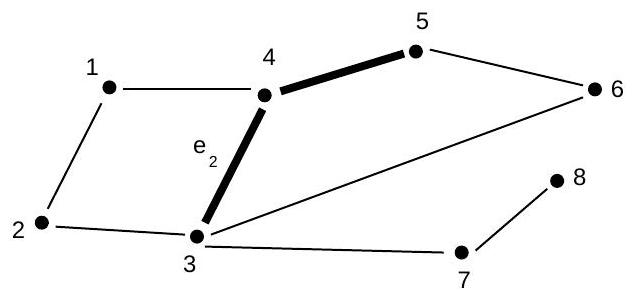
\includegraphics[max width=\textwidth, center]{2025_09_05_93c7c1835f249f70c0eeg-15(2)}

Como \#\{ ramas elegidas $\}=2<8-1=m-1$, repetimos 2 .\\
Elegimos $e_{3}$ ya que no forma ciclo con las ya elegidas.\\
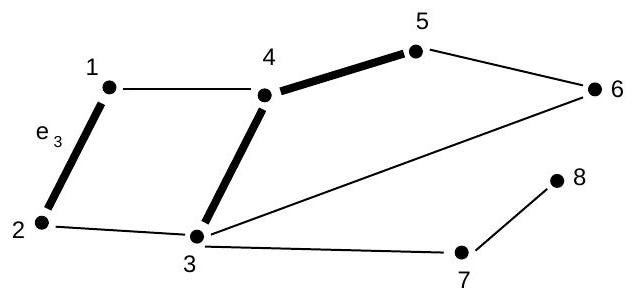
\includegraphics[max width=\textwidth, center]{2025_09_05_93c7c1835f249f70c0eeg-16(2)}

De la misma manera luego elegimos $e_{4}, e_{5}$ y $e_{6}$. Hasta ahora el gráfico es\\
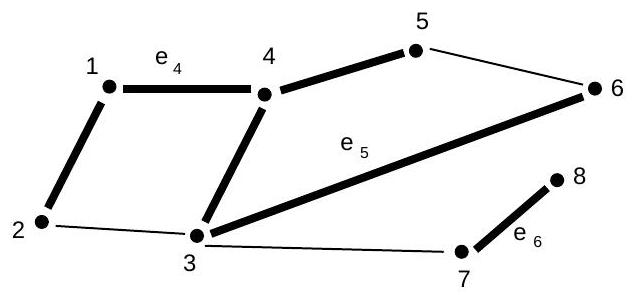
\includegraphics[max width=\textwidth, center]{2025_09_05_93c7c1835f249f70c0eeg-16}

Siendo que $\#\{$ ramas elegidas $\}=6<8-1=m-1$, repetimos 2 . Como $e_{7}$ y $e_{8}$ forman ciclo con las ya elegidas y $e_{9}$ no, elegimos $e_{9}$.\\
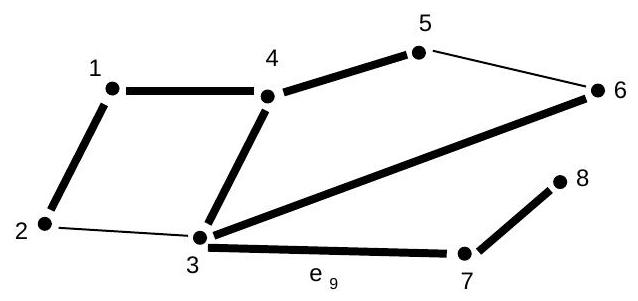
\includegraphics[max width=\textwidth, center]{2025_09_05_93c7c1835f249f70c0eeg-16(1)}

Como $\#\{$ ramas elegidas $\}=7=8-1=m-1$, STOP.\\
El grafo determinado por las líneas gruesas es un spanning tree mínimo de $G$.\\
Para demostrar la validez del algoritmo necesitaremos probar antes un resultado, que también utilizaremos luego para probar la validez del algoritmo de Prim que veremos en la sección 7.\\
Definición 6.2. Sea $G=(V, E)$ un grafo. Dado un subconjunto $A$ de $V$ definimos el conjunto

$$
\partial A=\{(u, v) \in E u \in A \text { y } v \in V-A\}
$$

El conjunto $\partial A$ se llama el corte definido por $A$.\\
Observación 6.3. Si $G$ es no dirigido entonces

$$
\partial A=\{e \in E / \text { un vértice de } e \text { pertenece a } A \text { y el otro a } V-A\}
$$

mientras que cuando $G$ es dirigido

$$
\partial A=\{e \in E / \text { la cola de } e \text { pertenece a } A \text { y la punta de } e \text { pertenece a } V-A\}
$$

Definición 6.4. Si $\partial A$ es un corte de $G$ y $U$ es un subconjunto de ramas de $G$, diremos que $U$ no cruza al corte $\partial A$ si $U \cap \partial A=\emptyset$.

Ejemplo 6.5. El conjunto $A=\{1,2,3,4\}$ define un corte en el grafo\\
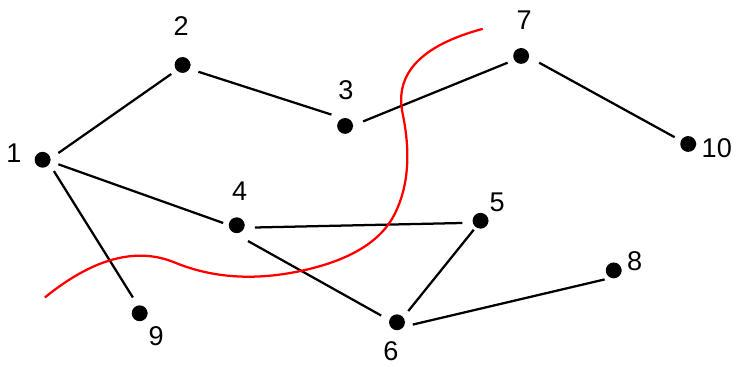
\includegraphics[max width=\textwidth, center]{2025_09_05_93c7c1835f249f70c0eeg-17(1)}

En la figura, $\partial A=\{(3,7),(4,5),(4,6),(1,9)\}$ es el conjunto de ramas intersecadas por la curva. El conjunto $U=\{(1,2),(5,6),(6,8)\}$ no cruza el corte.

Teorema 6.6. Sea $G=(V, E)$ un grafo no dirigido conexo, donde cada rama $e \in E$ tiene asignado un peso $\omega(e)$, y sea $\partial A$ un corte. Sea $U$ un subconjunto de ramas de un mínimo spanning tree $T$ de $G$ que no cruza el corte.\\
Si $e \in \partial A$ es una rama de mínimo peso entonces $U \cup\{e\}$ es un subconjunto de ramas de un mínimo spanning tree $T^{\prime}$ de $G$.

Demostración: Si $e$ es una rama de $T$ no hay nada que probar. Supongamos entonces que no lo es.\\
Como $T$ es conexo, si $e=(u, v)$ entonces existe un camino en $T$ de $u$ a $v$. Sean $e_{1}, \ldots, e_{r}$ las ramas de ese camino.\\
Ilustremos esta situación en un gráfico\\
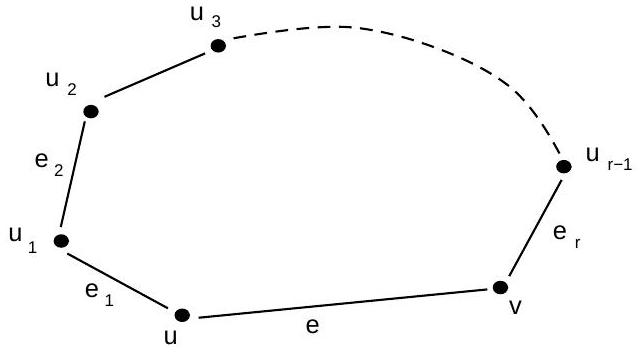
\includegraphics[max width=\textwidth, center]{2025_09_05_93c7c1835f249f70c0eeg-17}

Entonces existe $k$ tal que $e_{k} \in \partial A$. En efecto, como $e=(u, v) \in \partial A$ entonces $u \in A$ y $v \in V-A$. Luego si $u_{1} \notin A$ se sigue que $e_{1} \in \partial A$\\
si $u_{1} \in A$ y $u_{2} \notin A$ entonces $e_{2} \in \partial A$\\
$\vdots$\\
si $u_{r-2} \in A$ y $u_{r-1} \notin A$ entonces $e_{r-1} \in \partial A$\\
y, finalmente, si $u_{r-1} \in A$ entonces $e_{r} \in \partial A$ pues $v \notin A$.\\
Notemos que como $e_{k} \in \partial A$ y $U \cap \partial A=\emptyset$ ( $U$ no cruza el corte) entonces se tiene que $e_{k} \notin U$.\\
Sea $T^{\prime}$ el grafo que resulta de suprimir en $T$ la rama $e_{k}$ y agregar la rama $e$. Veamos que $T^{\prime}$ es un spanning tree de $G$. En efecto, como $T$ es conexo entonces $T^{\prime}$ también lo es. Sea $m=\# V$. Como $T$ es un spanning tree de $G$ entonces tiene $m-1$ ramas. Luego $T^{\prime}$ tiene $m-1$ ramas y $m$ vértices. Luego $T^{\prime}$ es un árbol por la proposición 2.10. y por lo tanto es un spanning tree de $G$. Además es mínimo porque $\omega(e) \leq \omega\left(e_{k}\right)$ (recordemos que $e$ era de mínimo peso en $\partial A$ y que $e_{k} \in \partial A$ ).\\
Así, $U \cup\{e\}$ es un subconjunto de ramas del spanning tree mínimo $T^{\prime}$ pues la rama $e_{k}$ que suprimimos no pertenecía a $U$.

\section*{Validez del algoritmo.}
Para cada $k$, consideremos el conjunto $U_{k}=\{$ ramas elegidas hasta la iteración $k\}$. Probaremos que, cualquiera sea $k, U_{k}$ es un subconjunto de ramas de un spanning tree mínimo $T_{k}$.\\
Iteración $k=0$ : En este caso $U_{0}=\emptyset$ y basta tomar $T_{0}$ como un spanning tree mínimo cualquiera.\\
Iteración $k=1$ : sea $U=U_{0}$ y sea $e_{1}=\left(u_{1}, v_{1}\right) \in E$ de mínimo peso. Entonces $U_{1}=U \cup\left\{e_{1}\right\}$.\\
Sea $\partial A_{1}$ el corte definido por $A_{1}=\left\{u_{1}\right\}$. Como $U$ un subconjunto de ramas de un mínimo spanning tree $T_{0}$ de $G$ que no cruza el corte y $e_{1} \in \partial A_{1}$ es de mínimo peso, entonces $U_{1}=U_{0} \cup\left\{e_{1}\right\}$ es un subconjunto de ramas de un spanning tree mínimo $T_{1}$ por el teorema 6.6.

Supongamos ahora que nuestra afirmación es cierta para $k$, es decir, que $U_{k}$ es un subconjunto de ramas de un spanning tree mínimo $T_{k}$.\\
Iteración $k+1$ : Sea $U=U_{k}$ y sea $e_{k+1}=\left(u_{k+1}, v_{k+1}\right) \notin U_{k}$ de mínimo peso entre las ramas que no pertenecen a $U_{k}$ y que no forman ciclo con las ya elegidas. Entonces $U_{k+1}=U \cup\left\{e_{k+1}\right\}$.\\
Sea

$$
A_{k+1}=\left\{v \in V / \exists \text { un camino en } U_{k} \text { de } v \text { a } u_{k+1}\right\} \cup\left\{u_{k+1}\right\}
$$

y sea $\partial A_{k+1}$ el corte definido por $A_{k+1}$.\\
Veamos que $U$ no cruza el corte, es decir, que $\partial A_{k+1} \cap U_{k}=\emptyset$. Supongamos que no. Sea $e \in \partial A_{k+1} \cap U_{k}$. Luego $e=(u, v)$ donde $u \in A_{k+1}, v \notin A_{k+1}$ y $(u, v)=e \in U_{k}$. Como $u \in A_{k+1}$ entonces $u=u_{k+1}$ o existe un camino en $U_{k}$ de $u$ a $u_{k+1}$.\\
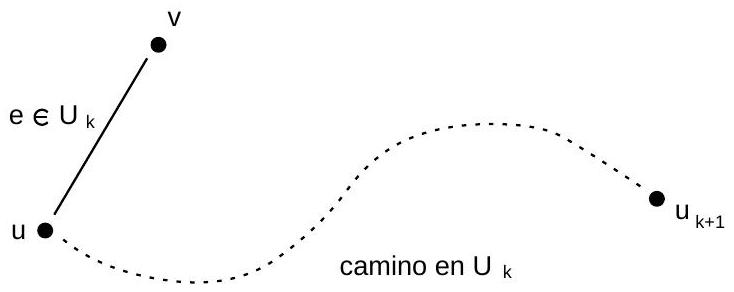
\includegraphics[max width=\textwidth, center]{2025_09_05_93c7c1835f249f70c0eeg-18(1)}

Luego, existe un camino en $U_{k}$ de $v$ a $u_{k+1}$. Absurdo, pues $v \notin A_{k+1}$.\\
Luego, $U$ es un subconjunto de ramas de un spanning tree mínimo $T_{k}$ que no cruza el corte.\\
Por otra parte, $e_{k+1} \in \partial A_{k+1}$. En efecto, $u_{k+1} \in A_{k+1}$ y $v_{k+1} \notin A_{k+1}$ ya que si existiera un camino en $U_{k}$ uniendo $v_{k+1}$ y $u_{k+1}$ entonces $e_{k+1}$ formaría un ciclo con las ramas ya elegidas.\\
Ahora veamos que $e_{k+1}$ es de mínimo peso en $\partial A_{k+1}$. Como $e_{k+1}$ fue elegida de mínimo peso entre las ramas que no pertenecían a $U_{k}$ y que no formaban ciclo con las ya elegidas, basta ver que toda rama en $\partial A_{k+1}$ no pertenece a $U_{k}$ y no forma ciclo con las ya elegidas.\\
Si $e \in \partial A_{k+1}$, entonces claramente $e$ no pertenece a $U_{k}$ pues $U_{k}=U$ no cruza el corte. Veamos que no forma ciclo con las ramas ya elegidas.\\
Si $e=(u, v)$ con $u \in A_{k+1}, v \notin A_{k+1}$ formara ciclo, entonces existiría un camino en $U_{k}$ uniendo $u$ y $v$. Además, existiría un camino en $U_{k}$ uniendo $u_{k+1}$ y $u$ pues $u \in A_{k+1}$.\\
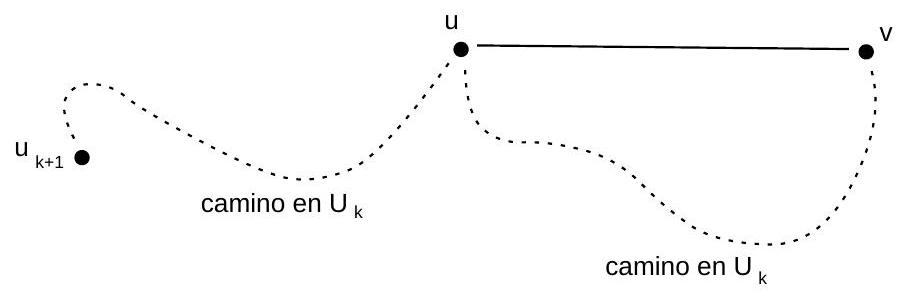
\includegraphics[max width=\textwidth, center]{2025_09_05_93c7c1835f249f70c0eeg-18}

Por lo tanto existiría un camino en $U_{k}$ uniendo $v$ y $u_{k+1}$, lo que contradice que $v \notin A_{k+1}$.

Luego, por el teorema 6.6., $U_{k+1}=U_{k} \cup\left\{e_{k+1}\right\}$ es un subconjunto de ramas de un spanning tree mínimo $T_{k+1}$.

Luego, para todo $k$, el conjunto de ramas elegidas hasta la $k$-ésima iteración es un subconjunto de ramas de un spanning tree mínimo $T_{k}$. Sea $m=\# V$. Como $\# U_{k}=k$ para todo $k$ ya que en cada iteración se agrega una rama ( $U_{k+1}=U_{k} \cup\left\{e_{k+1}\right\}$ con $e_{k+1} \notin U_{k}$ ) y el algoritmo se detiene cuando hay $m-1$ ramas elegidas, entonces el algoritmo se detiene cuando $k=m-1$. Además, $U_{m-1}$ será un conjunto de $m-1$ ramas que es un subconjunto de ramas de un spanning tree mínimo $T_{m-1}$. Pero como $T_{m-1}$ también tiene $m-1$ ramas por ser un spanning tree entonces se tiene que $U_{m-1}$ es igual al conjunto de ramas de $T_{m-1}$. Esto significa que si $E^{\prime}$ es el conjunto de las $m-1$ ramas elegidas por el algoritmo entonces $\left(V, E^{\prime}\right)=T_{m-1}$ y por lo tanto es un mínimo spanning tree de $G$.

Para aplicar el algoritmo de Kruskal debemos ordenar las ramas de menor a mayor costo. Hay muchos algoritmos que se pueden utilizar para ordenar. Veremos uno conocido como 'divide and conquer'.

\section*{Divide and conquer.}
Supongamos que queremos ordenar de menor a mayor los números $a_{1}, a_{2}, \ldots, a_{n}$.

\begin{enumerate}
  \item Partimos el conjunto $\left\{a_{1}, \ldots, a_{n}\right\}$ en los subconjuntos de $2=2^{1}$ elementos cada uno:
\end{enumerate}

$$
\left\{a_{1}, a_{2}\right\} \quad\left\{a_{3}, a_{4}\right\} \quad\left\{a_{5}, a_{6}\right\} \quad \cdots \cdots \cdot \quad \cdots \cdots \cdot \quad \cdots \cdots . \quad \cdots \cdots
$$

Ordenamos los elementos de cada uno de los subconjuntos de dos elementos.\\
2. Partimos el conjunto $\left\{a_{1}, \ldots, a_{n}\right\}$ en los subconjuntos de $4=2^{2}$ elementos cada uno:

$$
\left\{a_{1}, a_{2}, a_{3}, a_{4}\right\} \quad\left\{a_{5}, a_{6}, a_{7}, a_{8}\right\} \quad \cdots \cdots \cdot \quad \cdots \cdots \cdot \quad \cdots \cdots
$$

Ordenamos los elementos de cada uno de los subconjuntos de cuatro elementos teniendo en cuenta el orden obtenido en el paso previo.\\
3. Partimos el conjunto $\left\{a_{1}, \ldots, a_{n}\right\}$ en los subconjuntos de $8=2^{3}$ elementos cada uno:

$$
\left\{a_{1}, a_{2}, a_{3}, a_{4}, a_{5}, a_{6}, a_{7}, a_{8}\right\} \quad\left\{a_{9}, a_{10}, a_{11}, a_{12}, a_{13}, a_{14}, a_{15}, a_{16}\right\} \quad \cdots \cdots
$$

Ordenamos los elementos de cada uno de los subconjuntos de ocho elementos teniendo en cuenta el orden obtenido en el paso previo.\\
Seguimos de este modo hasta tener un solo subconjunto con los $n$ elementos ordenados.\\
Si $\left\{b_{1}, \ldots, b_{r}\right\}$ y $\left\{c_{1}, \ldots, c_{r}\right\}$ están ordenados, para ordenar $\left\{b_{1}, \ldots, b_{r}, c_{1}, \ldots, c_{r}\right\}$ (es decir, para ordenar cada subconjunto al pasar del paso $k$ al paso $k+1$ ) necesitamos hacer, a lo sumo, $2 r$ comparaciones. Veamos esto en un par de ejemplos y luego veamos el caso general.

Ejemplo 6.7 Supongamos que sabemos que $b_{1} \leq b_{2} \leq b_{3} \leq b_{4} \leq b_{5} \leq b_{6}$ y que $c_{1} \leq c_{2} \leq c_{3} \leq c_{4} \leq c_{5} \leq c_{6}$ y supongamos que el orden final sería

$$
b_{1}, b_{2}, c_{1}, b_{3}, c_{2}, b_{4}, b_{5}, c_{3}, b_{6}, c_{4}, c_{5}, c_{6}
$$

Entonces, para encontrar el orden final habremos tenido que comparar

$$
c_{1} \operatorname{con} b_{1}, b_{2}, b_{3}, \quad c_{2} \operatorname{con} b_{3}, b_{4}, \quad c_{3} \operatorname{con} b_{4}, b_{5}, b_{6} \quad y \quad c_{4} \operatorname{con} b_{6}
$$

Necesitamos $9 \leq 2.6$ comparaciones.

Ejemplo 6.8 Supongamos que sabemos que

$$
b_{1} \leq b_{2} \leq b_{3} \leq b_{4} \leq b_{5}
$$

y que

$$
c_{1} \leq c_{2} \leq c_{3} \leq c_{4} \leq c_{5}
$$

y supongamos que el orden final debe ser

$$
b_{1}, c_{1}, b_{2}, c_{2}, b_{3}, c_{3}, b_{4}, c_{4}, b_{5}, c_{5}
$$

Entonces, para encontrar el orden final habremos tenido que comparar

$$
c_{1} \operatorname{con} b_{1}, b_{2}, \quad c_{2} \operatorname{con} b_{2}, b_{3}, \quad c_{3} \operatorname{con} b_{3}, b_{4}, \quad c_{4} \operatorname{con} b_{4}, b_{5} \quad \text { y } \quad c_{5} \operatorname{con} b_{5}
$$

Necesitamos $9 \leq 2.5$ comparaciones. Veamos ahora el caso general.\\
Veremos que para ordenar el conjunto $\left\{b_{1}, \ldots, b_{r}, c_{1}, \ldots, c_{r}\right\}$, donde $b_{1} \leq b_{2} \leq \cdots \leq b_{r}$ y $c_{1} \leq c_{2} \leq \cdots \leq c_{r}$, se necesitan a lo sumo $2 r$ comparaciones. Sea $b_{0}=-\infty$ y sea $x_{j}$ definido por

$$
x_{j}= \begin{cases}r & \text { si } c_{j}>b_{r} \\ 1 & \text { si } j=0 \\ s & \text { si } b_{s-1}<c_{j} \leq b_{s},(1 \leq s \leq r)\end{cases}
$$

Entonces par ordenar $c_{j}$ se necesitan a lo sumo $x_{j}-x_{j-1}+1$ comparaciones ya que $c_{j}$ debe ser comparado con los $x_{j}-x_{j-1}+1$ números $b_{x_{j-1}}, \ldots, b_{x_{j}}$. En el ejemplo 6.7., para $j=3$ resulta que $x_{j-1}=x_{2}=4$ (pues $b_{3}<c_{2} \leq b_{4}$ ) y $x_{j}=x_{3}=6$ pues $b_{5}<c_{3} \leq b_{6}$ y por lo tanto $c_{j}=c_{3}$ debe ser comparado con $b_{x_{j-1}}, \ldots, b_{x_{j}}=b_{4}, b_{5}, b_{6}$.\\
Luego, en total necesitaremos a lo sumo

$$
x_{1}+\left(x_{2}-x_{1}+1\right)+\left(x_{3}-x_{2}+1\right)+\cdots+\left(x_{r}-x_{r-1}+1\right)=x_{r}+r-1 \leq 2 r
$$

comparaciones para ordenar cada subconjunto de $2 r$ elementos generado a partir de dos subconjuntos de $r$ elementos ordenados.

Por último, veamos que el algoritmo 'divide and conquer' para ordenar $n$ elementos tiene complejidad $O(n . \log n)$.\\
Para el primer paso necesitamos hacer $\frac{n}{2}$ comparaciones. Además, en cada paso $k$ tenemos $\frac{n}{2^{k}}$ subconjuntos de $2^{k}$ elementos cada uno que queremos ordenar, y cada uno de estos subconjuntos es la unión de dos conjuntos de $r=2^{k-1}$ elementos que ya están ordenados. Luego, necesitamos hacer $2 r=2.2^{k-1}$ comparaciones por cada uno de los $\frac{n}{2^{k}}$ subconjuntos, es decir, un total de $2^{k} \cdot \frac{n}{2^{k}}=n$\\
Si $2^{t-1}<n \leq 2^{t}$ entonces en $t \leq 1+\log n$ pasos terminamos ya que en el paso $k$ ordenamos subconjuntos de $2^{k}$ elementos. Como en cada paso hacemos a lo sumo $n$ comparaciones y se realizan a lo sumo $1+\log n \leq 2 \log n$ pasos entonces la complejidad de este algoritmo es $O(n \cdot \log n)$, donde log denota el logaritmo en base 2 .

\section*{Implementación del algoritmo de Kruskal.}
Supongamos que $V=\left\{v_{1}, \ldots, v_{m}\right\}$ y $E=\left\{e_{1}, \ldots, e_{n}\right\}$, donde hemos ordenado las ramas de manera que $e_{1}$ sea la de menor peso, $e_{2}$ a la que sigue, etc.\\
Ahora, en cada iteración debemos elegir una rama de mínimo peso entre las no elegidas que no forman ciclo con las que tenemos hasta ese momento. Para hacer esto en la forma en que una máquina pudiera hacerlo,\\
notemos que en la iteración $k$ del algoritmo, el grafo $\left(V, U_{k}\right)$, donde $U_{k}$ denota el conjunto de ramas elegidas hasta la $k$-ésima iteración, constituye una foresta con $m-k$ árboles. En cada iteración asignaremos a cada uno de estos árboles un número entre 1 y $m$ y llevaremos un registro de cuáles son los nodos y las ramas que lo forman.\\
Utilizaremos dos vectores $x=\left(x_{1}, \ldots, x_{m}\right)$ e $y=\left(y_{1}, \ldots, y_{n}\right)$ y una variable $t$. El valor de la coordenada $x_{i}$ de $x$ nos dirá el número de árbol al pertenece el nodo $v_{i}$ y el valor de la coordenada $y_{j}$ de $y$ nos dirá el número de árbol al que pertenece la rama $e_{j}$, o valdrá -1 si $e_{j}$ no fue examinada aún, o valdrá 0 si $e_{j}$ fue examinada y descartada porque formaba ciclo con las ramas ya elegidas. El valor de la variable $t$ nos indicará cuál es la rama que nos toca examinar. Además, utilizaremos un contador $c$ que nos indicará cuál es la iteración que hemos realizado. El algoritmo se detendrá cuando $c$ valga $m-1$.

En la iteración cero inicializamos las variables $c$ y $t$ poniendo $c=0, t=1$ y los vectores $x$ e $y$ en la forma $x_{1}=1, x_{2}=2, \ldots, x_{m}=m, y_{1}=-1, y_{2}=-1, \ldots, y_{n}=-1$. Esta asignación corresponde a la foresta inicial formada por los $m$ vértices y ninguna rama.\\
Supongamos que hemos realizado las primeras $k$ iteraciones. En este momento $c=k$ y la foresta puede describirse como sigue: cada árbol de la foresta está formado por las ramas y vértices cuyas correspondientes coordenadas en los vectores $x$ e $y$ tienen un mismo número positivo. Si $y_{j}>0$ significa que la rama $e_{j}$ fue elegida, si $y_{j}=0$ significa que la rama $e_{j}$ fue examinada y descartada porque formaba ciclo con las ya elegidas y si $y_{j}=-1$ significa que la rama $e_{j}$ aún no fue examinada. El valor que tiene $t$ en este momento nos indica cuál es la primera rama que debemos examinar al comenzar la iteración $k+1$.\\
Iteración $k+1$ : examinamos la rama $e_{t}$. Supongamos que $e_{t}=\left(v_{i}, v_{j}\right)$. Para ver si forma un ciclo con las ramas de la foresta actual comparamos los dos valores de $x_{i}$ y $x_{j}$ correspondientes a los vértices $v_{i}$ y $v_{j}$ de $e_{t}$. Si son distintos, entonces estos vértices pertenecen a distintos árboles y por lo tanto agregar la rama fusionará esos árboles formando uno nuevo y no habrá ciclo. Pero si son iguales, entonces pertenecen a un mismo árbol. Como el árbol es conexo existe un camino en él de $v_{i}$ a $v_{j}$ y por lo tanto agregar la rama formará ciclo con las ya elegidas.\\
Si vemos que $e_{t}$ forma ciclo, actualizamos el valor de $y_{t}$ poniendo $y_{t}=0$ para indicar que la rama $e_{t}$ fue examinada y descartada, actualizamos $t$ en la forma $t=t+1$ y pasamos a examinar la rama $e_{t}$. Si en cambio no forma ciclo, el agregar esa rama fusionará los árboles $x_{i}$ y $x_{j}$. Supongamos que el valor de $x_{i}$ es $r$ y el de $x_{j}$ es $s$, con $s<r$. Entonces actualizamos los vectores $x$ e $y$ poniendo $y_{t}=s, x_{l}=s \forall l / x_{l}=r$, $y_{l}=s \forall l / y_{l}=r$. Esto indica que ahora el árbol $s$ está formado por todos los vértices y ramas que tenía hasta ese momento, la rama $e_{t}$ y todos los vértices y ramas que antes pertenecían al árbol $s$. Además, actualizamos $t$ y $c$ en la forma $t=t+1$ y $c=c+1$.\\
Repetimos este procedimiento hasta que $c=m-1$, es decir, hasta que haya $m-1$ ramas elegidas (notemos que en cada iteración elegimos una rama). En ese momento todas las coordenadas de $x$ valdrán 1 y las coordenadas de $y$ valdrán $0,1 \mathrm{o}-1$. Más aún, habrá exactamente $m-1$ coordenadas de $y$ que tengan el valor 1. Esas son las coordenadas que corresponden a las $m-1$ ramas del mínimo spanning tree buscado.

Ejemplo 6.9. Aplicaremos el algoritmo de Kruskal al grafo con $m=7$ vértices\\
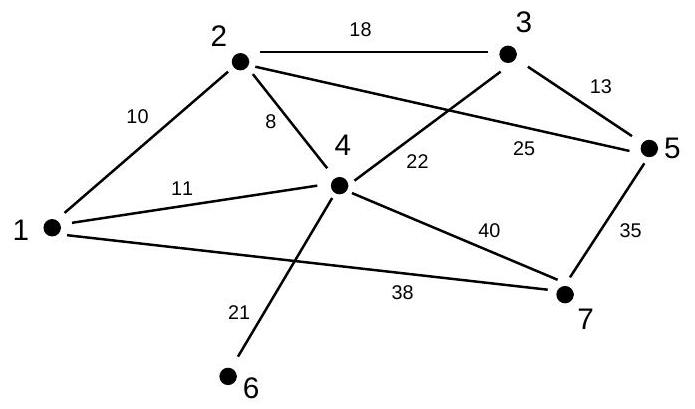
\includegraphics[max width=\textwidth, center]{2025_09_05_93c7c1835f249f70c0eeg-21}\\
para obtener un mínimo spanning tree. Primero ordenamos las ramas de menor a mayor según el peso:

\begin{center}
\begin{tabular}{|c|c|}
\hline
$e$ & $\omega(e)$ \\
\hline
$e_{1}=(2,4)$ & $\omega\left(e_{1}\right)=8$ \\
\hline
$e_{2}=(1,2)$ & $\omega\left(e_{2}\right)=10$ \\
\hline
$e_{3}=(1,4)$ & $\omega\left(e_{3}\right)=11$ \\
\hline
$e_{4}=(3,5)$ & $\omega\left(e_{4}\right)=13$ \\
\hline
$e_{5}=(2,3)$ & $\omega\left(e_{5}\right)=18$ \\
\hline
$e_{6}=(6,4)$ & $\omega\left(e_{6}\right)=21$ \\
\hline
$e_{7}=(4,3)$ & $\omega\left(e_{7}\right)=22$ \\
\hline
$e_{8}=(2,5)$ & $\omega\left(e_{8}\right)=25$ \\
\hline
$e_{9}=(5,7)$ & $\omega\left(e_{9}\right)=35$ \\
\hline
$e_{10}=(1,7)$ & $\omega\left(e_{10}\right)=38$ \\
\hline
$e_{11}=(4,7)$ & $\omega\left(e_{11}\right)=40$ \\
\hline
\end{tabular}
\end{center}

En la siguiente tabla se ven las actualizaciones de los vectores $x$ e $y$, donde $x_{i}$ corresponde al vértice $i$ e $y_{j}$ a la rama $e_{j}$ y el estado del contador $c$.

\begin{center}
\begin{tabular}{|l|l|l|l|l|l|l|l|}
\hline
c & 0 & 1 & 2 & 3 & 4 & 5 & 6 \\
\hline
$x_{1}$ & 1 & 1 & 1 & 1 & 1 & 1 & 1 \\
\hline
$x_{2}$ & 2 & 2 & 1 & 1 & 1 & 1 & 1 \\
\hline
$x_{3}$ & 3 & 3 & 3 & 3 & 1 & 1 & 1 \\
\hline
$x_{4}$ & 4 & 2 & 1 & 1 & 1 & 1 & 1 \\
\hline
$x_{5}$ & 5 & 5 & 5 & 3 & 1 & 1 & 1 \\
\hline
$x_{6}$ & 6 & 6 & 6 & 6 & 6 & 1 & 1 \\
\hline
$x_{7}$ & 7 & 7 & 7 & 7 & 7 & 7 & 1 \\
\hline
$y_{1}$ & -1 & 2 & 1 & 1 & 1 & 1 & 1 \\
\hline
$y_{2}$ & -1 & -1 & 1 & 1 & 1 & 1 & 1 \\
\hline
$y_{3}$ & -1 & -1 & -1 & 0 & 0 & 0 & 0 \\
\hline
$y_{4}$ & -1 & -1 & -1 & 3 & 1 & 1 & 1 \\
\hline
$y_{5}$ & -1 & -1 & -1 & -1 & 1 & 1 & 1 \\
\hline
$y_{6}$ & -1 & -1 & -1 & -1 & -1 & 1 & 1 \\
\hline
$y_{7}$ & -1 & -1 & -1 & -1 & -1 & -1 & 0 \\
\hline
$y_{8}$ & -1 & -1 & -1 & -1 & -1 & -1 & 0 \\
\hline
$y_{9}$ & -1 & -1 & -1 & -1 & -1 & -1 & 1 \\
\hline
$y_{10}$ & -1 & -1 & -1 & -1 & -1 & -1 & -1 \\
\hline
$y_{11}$ & -1 & -1 & -1 & -1 & -1 & -1 & -1 \\
\hline
\end{tabular}
\end{center}

Ahora analicemos cómo es la foresta en cada iteración del algoritmo. En la interación cero la foresta inicial consiste de siete árboles, cada uno de ellos formado por un único vértice y ninguna rama.\\
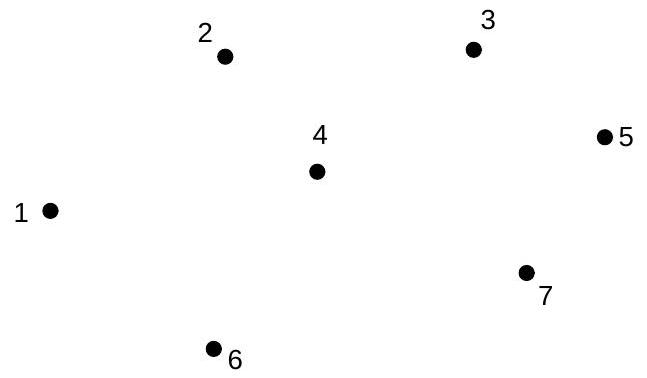
\includegraphics[max width=\textwidth, center]{2025_09_05_93c7c1835f249f70c0eeg-22}

En este momento se tiene que $t=1$ y $c=0$.

Primera iteración: como $t=1$ examinamos la rama $e_{1}$. Se comparan los valores de $x_{2}$ y $x_{4}$ correspondientes a los vértices 2 y 4 que son los extremos de la rama de menor peso $e_{1}$.\\
Como $x_{2}=2 \neq 4=x_{4}$ entonces actualizamos los vectores $x$ e $y$ poniendo $x_{2}=2=x_{4}$ e $y_{1}=2$. Esto significa que la rama $e_{1}$ fue elegida y, al agregarla, los árboles 2 y 4 se fusionaron formando un solo árbol, el árbol 2.\\
Ahora la foresta tiene seis árboles, cinco de ellos (los árboles $1,3,5,6$ y 7 ) formados por un vértice y ninguna rama y el otro (el árbol 2) por los vértices 2 y 4 y la rama $e_{1}$.\\
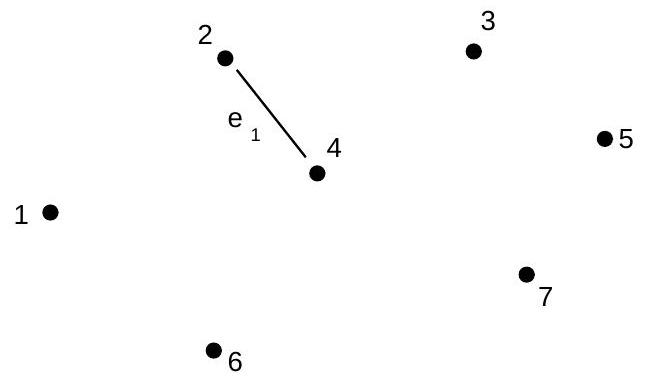
\includegraphics[max width=\textwidth, center]{2025_09_05_93c7c1835f249f70c0eeg-23}

Actualizamos los valores de $t$ y $c$ poniendo $t=2$ y $c=1$.\\
Segunda iteración: como $t=2$ se comparan los valores de $x_{1}$ y $x_{2}$ correspondientes a los vértices 1 y 2 que son los extremos de la rama $e_{2}$ (que es la de menor peso entre las no elegidas hasta el momento).\\
Como $x_{1}=1 \neq 2=x_{2}$ entonces actualizamos los vectores $x$ e $y$ poniendo $x_{2}=1, x_{4}=1, y_{1}=1$ e $y_{2}=1$.\\
Esto significa que la rama $e_{2}$ fue elegida y al agregarla se fusionaron los árboles 1 y 2 formando un solo árbol, el árbol 1 .\\
Ahora la foresta tiene cinco árboles. Cuatro de ellos (los árboles $3,5,6$ y 7 ) están formados por un vértice y ninguna rama y el otro (el árbol 1) está formado por los vértices 1,2 y 4 y las ramas $e_{1}$ y $e_{2}$.\\
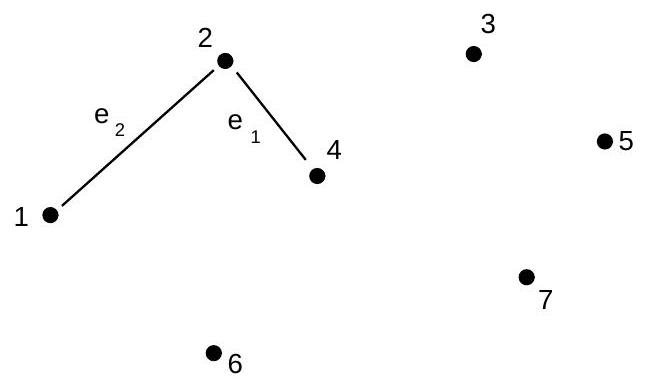
\includegraphics[max width=\textwidth, center]{2025_09_05_93c7c1835f249f70c0eeg-23(1)}

Actualizamos los valores de $t$ y $c$ poniendo $t=3$ y $c=2$.\\
Tercera iteración: como $t=3$, se comparan los valores de $x_{1}$ y $x_{4}$ correspondientes a los vértices 1 y 4 que son los extremos de la rama $e_{3}$ (que es la de menor peso entre las no elegidas hasta el momento).\\
Como $x_{1}=2=x_{4}$ entonces actualizamos los vectores $x$ e $y$ poniendo $y_{3}=0$. Esto significa que la rama $e_{3}$ fue descartada pues formaba ciclo con las ya elegidas. Ahora actualizamos $t$ poniendo $t=4$. Como $t=4$, se comparan los valores de $x_{3}$ y $x_{5}$ correspondientes a los vértices 3 y 5 que son los extremos de la rama $e_{4}$ (que es la de menor peso entre las no elegidas hasta el momento). Como $x_{3}=3 \neq 5=x_{5}$ entonces actualizamos los vectores $x$ e $y$ poniendo $x_{3}=3, x_{5}=3$ e $y_{4}=3$. Esto significa que la rama $e_{4}$ fue elegida y al agregarla se fusionaron los árboles 3 y 5 fomando un solo árbol, el árbol 3 .\\
Ahora la foresta tiene cuatro árboles. Dos de ellos (los árboles 6 y 7 ) formados por un vértice y ninguna rama, el árbol 1 formado por los vértices 1,2 y 4 y las ramas $e_{1}$ y $e_{2}$ y el árbol 3 por los vértices 3 y 5 y la rama $e_{4}$.\\
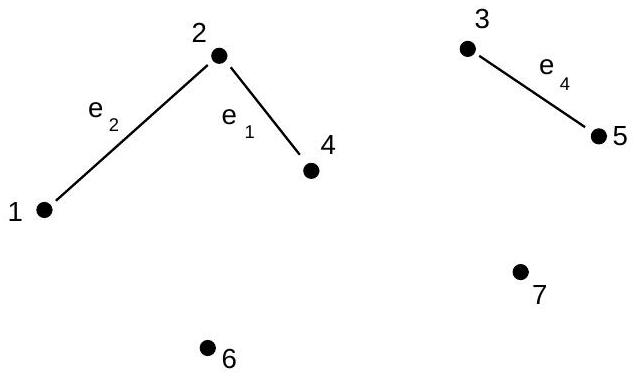
\includegraphics[max width=\textwidth, center]{2025_09_05_93c7c1835f249f70c0eeg-24(1)}

Actualizamos los valores de $t$ y $c$ poniendo $t=5$ y $c=3$.\\
De manera análoga se ve que la foresta en las restantes iteraciones es como sigue\\
Foresta en la cuarta iteración, donde se fusionan los árboles 1 y 3 al agregar la rama $e_{5}$\\
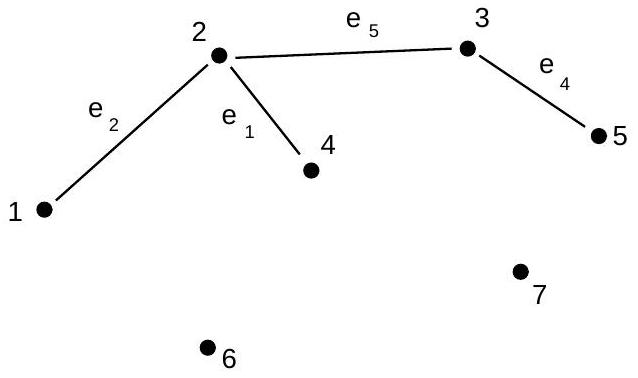
\includegraphics[max width=\textwidth, center]{2025_09_05_93c7c1835f249f70c0eeg-24(3)}

Foresta en la quinta iteración, donde se fusionan los árboles 1 y 6 al agregar la rama $e_{6}$\\
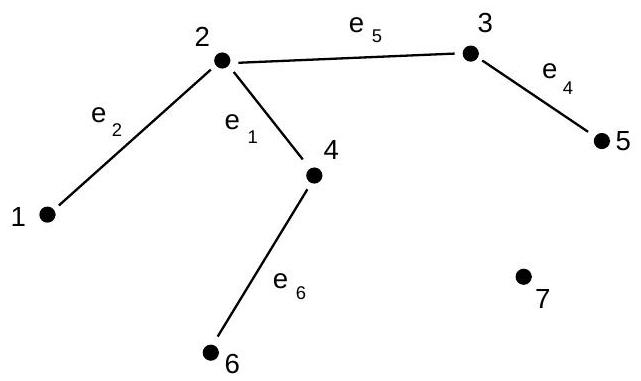
\includegraphics[max width=\textwidth, center]{2025_09_05_93c7c1835f249f70c0eeg-24}

Foresta en la sexta iteración, donde las ramas $e_{7}$ y $e_{8}$ son descartadas y se fusionan los árboles 1 y 7 al agregar la rama $e_{9}$\\
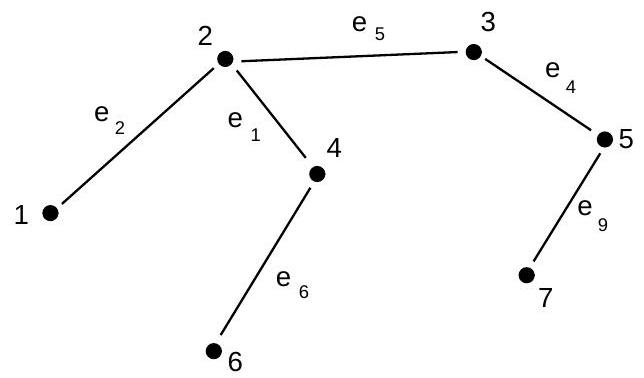
\includegraphics[max width=\textwidth, center]{2025_09_05_93c7c1835f249f70c0eeg-24(2)}

Este es el mínimo spanning tree de $G$ buscado.

\section*{Complejidad del algoritmo.}
Sean $m=\# V$ y $n=\# E$. Como en la primera iteración se ordenan las $n$ ramas y además, en cada iteración\\
se hacen a lo sumo c.n comparaciones y actualizaciones (donde $c$ es una constante) y se realizan a lo sumo $m$ iteraciones, entonces la complejidad de este algoritmo es $O(n \cdot \log n)+m \cdot O(n)$.\\
Dado que $n \leq\binom{ m}{2} \leq m^{2}$, entonces $n \cdot \log n \leq n \cdot \log m^{2}=2 n \cdot \log m \leq 2 n \cdot m$. Por lo tanto la compeljidad es $O(n . m)$, es decir, es menor o igual que $k . n . m$ para una constante $k$. Como en el caso del algorimto search, este algoritmo es polinomial. En efecto, si $N$ es el tamaño del input, se tiene que $n+m \leq N$. Luego $n . m \leq(n+m)^{2} \leq N^{2}$ de donde la complejidad del algoritmo es menor o igual que $P(N)$ donde $P$ es el polinomio $k X^{2}$.

\section*{7. El algoritmo de Prim.}
Sea $G=(V, E)$ un grafo no dirigido, conexo, donde cada rama $e \in E$ tiene asignado un peso $\omega(e)$ y sea $m=\# V$. Describiremos ahora otro algoritmo, conocido como el algoritmo de Prim que también encuentra, en tiempo polinomial, un spanning tree mínimo de $G$. Dejamos como ejercicio el cálculo de su complejidad.

\section*{Descripción del algoritmo.}
\begin{enumerate}
  \item Ordenar las ramas de $G$ de menor a mayor según el peso.
  \item Elegir un vértice inicial cualquiera $u_{0}$.
  \item Sea $U$ el subárbol formado hasta ahora. Añadir una rama $(u, v)$ a $U$ de peso mínimo entre aquellas ramas no pertenecientes a $U$ que agregadas a $U$ forman un subárbol de $G$.
  \item repetir 3. si el número de ramas del subárbol formado hasta ahora es menor que $m-1$.
\end{enumerate}

\section*{Validez del algoritmo.}
Dejamos a cargo del lector justificar la validez de este algoritmo. La demostración es análoga a la de la validez del algoritmo de Kruskal. Debe probarse que, para cada $k, U_{k}=\{$ ramas elegidas hasta el paso $k\}$ es un subconjunto de un spanning tree mínimo $T_{k}$.

Sugerencia: para el paso cero tomar $U_{0}=\emptyset, T_{0}$ un spanning tree mínimo y, para el paso inductivo, aplicar el teorema 6.6. a $U=U_{k}=\{$ ramas del subárbol formado hasta ahora $\}$ y al corte definido por el conjunto $A_{k+1}=\{$ vértices del subárbol formado hasta ahora $\}$.\\
Notar que entonces $\partial A_{k+1}=\{e \in E-U / U \cup\{e\}$ es un subárbol de $G\}$.\\
Ejemplo 7.1. Apliquemos el algoritmo de Prim al siguiente grafo, donde en cada rama hemos indicado su peso\\
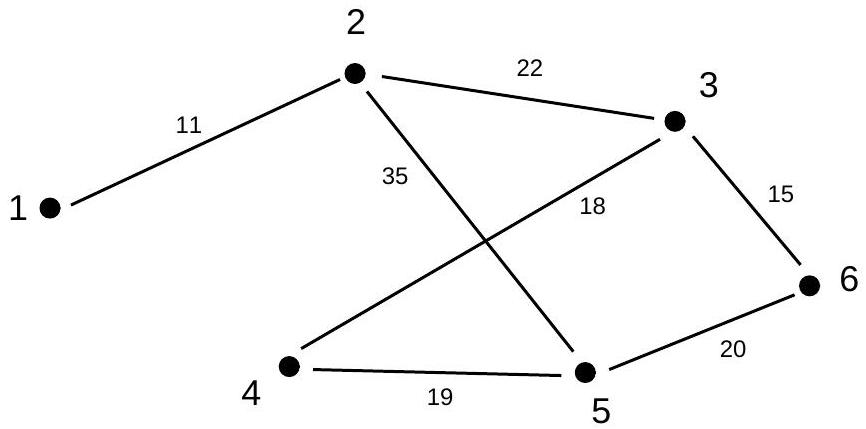
\includegraphics[max width=\textwidth, center]{2025_09_05_93c7c1835f249f70c0eeg-25}

Se tiene\\
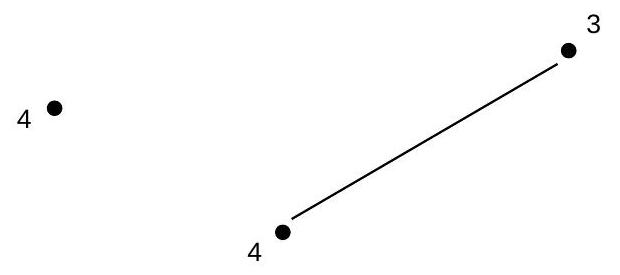
\includegraphics[max width=\textwidth, center]{2025_09_05_93c7c1835f249f70c0eeg-26(4)}\\
\includegraphics[max width=\textwidth, center]{2025_09_05_93c7c1835f249f70c0eeg-26(1)}\\
\includegraphics[max width=\textwidth, center]{2025_09_05_93c7c1835f249f70c0eeg-26(2)}\\
\includegraphics[max width=\textwidth, center]{2025_09_05_93c7c1835f249f70c0eeg-26}\\
\includegraphics[max width=\textwidth, center]{2025_09_05_93c7c1835f249f70c0eeg-26(3)}

\section*{8. El camino óptimo en un grafo dirigido.}
Sea $G=(V, E)$ un grafo dirigido y supongamos que para cada rama $e=(u, v) \in E$ tenemos definido un costo (o distancia) $c_{e}=c_{u v}$.\\
Si $\mathcal{P}$ es un camino dirigido en $G$ definimos el costo de $\mathcal{P}$ como la suma de los costos de las ramas que lo forman. Fijado un vértice $s$ queremos encontrar, para cada vértice $v$ de $G$, un camino dirigido óptimo (i.e., de mínimo costo o distancia) de $s$ a $v$. En esta sección analizaremos varios algoritmos que resuelven este problema, pero antes veamos su utilidad en un ejemplo.\\
Ejemplo 8.1. Una empresa es contratada para reparar 100 torres eléctricas, para lo cual necesitará comprar barras de acero de distintas longitudes $L_{1}<L_{2}<\cdots<L_{n}$ cuya única diferencia es la longitud. La empresa compra estas barras a un fabricante, quien está dispuesto a venderle barras de cualquier longitud siempre y cuando compre un mínimo de 100 barras de cada longitud. Por lo tanto, a la empresa no le conviene comprar barras de todas las $n$ longitudes. En lugar de esto, le conviene comprar barras de ciertas longitudes y obtener las barras de cada longitud $L_{i}$ que no tiene cortando las barras de longitud más chica entre aquellas que tiene y cuya longitud es mayor que $L_{i}$. Por ejemplo, si necesita 10 barras de longitud $L_{1}, 5$ de longitud $L_{2}$ y 90 de longitud $L_{3}$, le conviene comprar 105 barras de longitud $L_{3}$ y cortar 10 de ellas para obtener las barras de longitud $L_{1}$ y 5 de ellas para obtener las barras de longitud $L_{2}$ en lugar de comprar 100 barras de longitud $L_{1}, 100$ de longitud $L_{2}$ y 100 de longitud $L_{3}$. En cambio, si necesita 99 barras de longitud $L_{1}, 20$ de longitud $L_{2}$ y 90 de longitud $L_{3}$, entonces le conviene comprar 100 de longitud $L_{1}$ y 110 de longitud $L_{3}$. Se plantea entonces el problema de elegir cuáles longitudes conviene comprar de manera de poder obtener las restantes por recorte, a un costo mínimo. Como $L_{n}>L_{i} \forall i$, la longitud $L_{n}$ debe ser una de las que se compren ya que no puede obtenerse por recorte de ninguna otra.\\
Para cada $i$ entre 1 y $n$ sea $c_{i}$ el costo de una barra de longitud $L_{i}$ y sea $p_{i}$ la cantidad de barras de longitud $L_{i}$ que necesitará la empresa para reparar las 100 torres.

Consideremos el grafo dirigido $G=(V, E)$, donde $V=\{0,1,2, \ldots, n\}$ y $E=\{(i, j) / 0 \leq i<j \leq n\}$. Por ejemplo, para $n=4$ el grafo sería\\
\includegraphics[max width=\textwidth, center]{2025_09_05_93c7c1835f249f70c0eeg-27}

Asignemos a cada rama $(i, j)(0 \leq i<j \leq n)$ el costo $c_{i j}=\max \left\{100, p_{i+1}+p_{i+2}+\cdots+p_{j}\right\} c_{j}$. Supongamos que $\mathcal{P}$ es un camino dirigido de 0 a $n$ y que los vértices de ese camino son $0, j_{1}, \ldots, j_{r}, n$. Entonces, si elegimos comprar las longitudes $L_{j_{1}}, \ldots, L_{j_{r}}$ y $L_{n}$ y obtener las restantes por recorte, resulta que el costo total de la compra determinado por esta elección es el costo de $\mathcal{P}$. En efecto, si $\mathcal{P}$ es el camino dirigido $\left(0, j_{1}\right),\left(j_{1}, j_{2}\right), \ldots,\left(j_{r-1}, j_{r}\right),\left(j_{r}, n\right)$ el costo de $\mathcal{P}$ es

$$
c_{0 j_{1}}+c_{j_{1} j_{2}}+\cdots+c_{j_{r-1} j_{r}}+c_{j_{r} n}
$$

Dado que de cada longitud deben comprarse un mínimo de 100 barras, entonces el costo de comprar $k$ barras de una dada longitud $L_{j}$ es $\max \{100, k\} c_{j}$. Luego, el costo de $\mathcal{P}$ es el costo de comprar $p_{1}+p_{2}+\cdots+p_{j_{1}}$ barras de longitud $L_{j_{1}}+$ el costo de comprar $p_{j_{1}+1}+p_{j_{1}+2}+\cdots+p_{j_{2}}$ barras de longitud $L_{j_{2}}+\cdots+$ el costo de comprar $p_{j_{r-1}+1}+p_{j_{r-1}+2}+\cdots+p_{j_{r}}$ barras de longitud $L_{j_{r}}+$ el costo de comprar $p_{1+j_{r}}+p_{2+j_{r}}+\cdots+p_{n}$ barras de longitud $L_{n}$. Luego el problema se resuelve hallando el camino dirigido de mínimo costo de 0 a $n$ en $G$. Si el camino de mínimo costo es

$$
0 \longrightarrow j_{1} \longrightarrow j_{2} \longrightarrow \cdots \longrightarrow j_{r} \longrightarrow n
$$

entonces a la empresa le conviene comprar max $\left\{100, p_{1}+p_{2}+\cdots+p_{j_{1}}\right\}$ barras de longitud $L_{j_{1}}$ y obtener las de longitudes menores que $L_{j_{1}}$ recortando las de longitud $L_{j_{1}}$, $\max \left\{100, p_{j_{1}+1}+p_{j_{1}+2}+\cdots+p_{j_{2}}\right\}$ barras de longitud $L_{j_{2}}$ y obtener las de longitudes mayores que $L_{j_{1}}$ y menores que $L_{j_{2}}$ recortando las de longitud $L_{j_{2}}, \ldots, \max \left\{100, p_{j_{r-1}+1}+p_{j_{r-1}+2}+\cdots+p_{j_{r}}\right\}$ barras de longitud $L_{j_{r}}$ y obtener las de longitudes mayores que $L_{j_{r-1}}$ y menores que $L_{j_{r}}$ recortando las de longitud $L_{j_{r}}$ y $\max \left\{100, p_{1+j_{r}}+p_{2+j_{r}}+\cdots+p_{n}\right\}$ barras de longitud $L_{n}$ y obtener las de longitudes mayores que $L_{j_{r}}$ y menores que $L_{n}$ recortando las de longitud $L_{n}$.

Sea $G$ un grafo dirigido donde cada rama ( $u, v$ ) tiene asignado un costo $c_{u v}$ y donde se ha fijado un vértice $s$.\\
Describiremos a continuación varios algoritmos que encuentran (cuando existe) el camino dirigido óptimo de $s$ a $u$ y su costo, para cualquier vértice $u \neq s$.

Observación 8.2. Sea $\mathcal{R}$ es un camino óptimo de $s$ a $u$ y sea $v$ el vértice anterior a $u$ en ese camino. Si $\mathcal{P}$ la parte de ese camino que va de $s$ a $v$ entonces $\mathcal{P}$ es un camino óptimo a $v$.\\
En efecto, si hubiera un camino más "barato" de $s$ a $v$, entonces ese camino seguido de la rama $(v, u)$ sería un camino más "barato" que el camino que resulta de agregar a $\mathcal{P}$ la rama ( $v, u$ ), es decir, más "barato" que el camino óptimo $\mathcal{R}$.

\section*{Método de programación dinámica.}
Para poder aplicar este método necesitaremos que el grafo $G$ no contenga ciclos dirigidos. Sea entonces $G=(V, E)$ un grafo que no contiene ciclos dirigidos, donde cada rama ( $u, v$ ) tiene asignado un costo $c_{u v} \mathrm{y}$\\
supongamos que el vértice fijado $s$ de $G$ es tal que de él sólo salen flechas. A este vértice $s$ lo llamaremos la fuente.\\
Claramente podemos suponer que $V=\{1,2, \ldots, m\}$. Para cada $i<j$ tal que $(i, j) \notin E$ tomaremos $c_{i j}=\infty$. Supondremos además que los vértices están numerados de 1 a $m$ de forma tal que valga

$$
(i, j) \in E \Longrightarrow i<j
$$

Dejamos como tarea para el lector probar que si $G$ no contiene ciclos dirigidos siempre es posible renumerar los vértices de manera que esto se verifique.\\
Luego, $s=1$ y vale $\{i /(i, j) \in E\} \subseteq\{1,2, \ldots, j-1\}$. Sea

$$
y_{j}= \begin{cases}0 & \text { si } j=1 \\ \infty & \text { si } j \geq 2 \text { y } \nexists \text { camino dirigido de } 1 \text { a } j \\ \text { costo de un camino dirigido óptimo de } 1 \text { a } j & \text { en otro caso }\end{cases}
$$

(Notar que, como el grafo no contiene ciclos dirigidos, si existe un camino dirigido a $j$ entonces existe un camino dirigido óptimo a $j$ )

Luego, para todo $i<j$ es $y_{j} \leq y_{i}+c_{i j}$. En efecto, esto es obvio si $(i, j) \in E$. Pero si $(i, j) \notin E$ entonces también vale pues en ese caso $c_{i j}=\infty$. Más aún, por la observación 8.2., si $i$ es el vértice anterior a $j$ en un camino dirigido óptimo de 1 a $j$, entonces $y_{j}=y_{i}+c_{i j}$.\\
Esto muestra que

$$
y_{j}=\min _{1 \leq i \leq j-1}\left\{y_{i}+c_{i j}\right\}
$$

y que si $k$ es el índice que realiza el mínimo entonces $k$ es el vértice anterior a $j$ en un camino óptimo de 1 a $j$.

\section*{Descripción del algoritmo.}
\begin{enumerate}
  \item $y_{1}=0, \mathrm{j}=2$.
  \item $y_{j}=\min _{1 \leq i \leq j-1}\left\{y_{i}+c_{i j}\right\}$. Si $y_{k}+c_{k j}=\min _{1 \leq i \leq j-1}\left\{y_{i}+c_{i j}\right\}$ poner $p_{j}=k$.
  \item $j=j+1$. Si $j \leq m$ ir a 2 .
\end{enumerate}

\section*{4. STOP}
Como $p_{j}$ es el índice que realiza el mínimo entonces es el predecesor a $j$ en un camino óptimo. Luego, conociendo $p_{j}$ para cada $2 \leq j \leq m$ podemos reconstruír ese camino.

Ejemplo 8.3. Apliquemos el algoritmo al grafo\\
\includegraphics[max width=\textwidth, center]{2025_09_05_93c7c1835f249f70c0eeg-28}\\
donde para cada rama $(i, j)$ hemos indicado su costo $c_{i j}$. Notemos que este grafo no contiene ciclos dirigidos y satisface $(i, j) \in E \Longrightarrow i<j$\\
$y_{1}=0$\\
$y_{2}=21, p_{2}=1$\\
$y_{3}=\min \left\{y_{1}+c_{13}, y_{2}+c_{23}\right\}$. Como $y_{1}+c_{13}=13$ e $y_{2}+c_{23}=\infty$ entonces $y_{3}=13, p_{3}=1$.\\
$y_{4}=\min \left\{y_{1}+c_{14}, y_{2}+c_{24}, y_{3}+c_{34}\right\}$. Como $y_{1}+c_{14}=\infty, y_{2}+c_{24}=33$ e $y_{3}+c_{34}=15$ entonces $y_{4}=15$, $p_{4}=3$.\\
$y_{5}=\min \left\{y_{1}+c_{15}, y_{2}+c_{25}, y_{3}+c_{35}, y_{4}+c_{45}\right\}$. Como $y_{1}+c_{15}=\infty, y_{2}+c_{25}=\infty, y_{3}+c_{35}=17$ e $y_{4}+c_{45}=16$ entonces $y_{5}=16, p_{5}=4$.\\
$y_{6}=\min \left\{y_{1}+c_{16}, y_{2}+c_{26}, y_{3}+c_{36}, y_{4}+c_{46}, y_{5}+c_{56}\right\}$. Como $y_{1}+c_{16}=\infty, y_{2}+c_{26}=\infty, y_{3}+c_{36}=\infty$, $y_{4}+c_{46}=10$ e $y_{5}+c_{56}=23$ entonces $y_{6}=10, p_{6}=4$.\\
Análogamente $y_{7}=14, p_{7}=5, y_{8}=10$ y $p_{8}=7$.\\
En el camino óptimo de 1 a 7 el predecesor de 7 es $p_{7}=5$, el de 5 es $p_{5}=4$, el de 4 es $p_{4}=3$ y el de 3 es $p_{3}=1$. Luego, el camino dirigido óptimo de 1 a 7 es $1 \longrightarrow 3 \longrightarrow 4 \longrightarrow 5 \longrightarrow 7$ con costo $y_{7}=14$. Análogamente el camino dirigido óptimo de 1 a 6 es $1 \longrightarrow 3 \longrightarrow 4 \longrightarrow 6$ con costo $y_{6}=10$.

\section*{Método de Dijkstra.}
Este método sólo se podrá aplicar en el caso en que los $\operatorname{costos} c_{e}=c_{u v}$ son no negativos para toda rama $e=(u, v)$. Si el grafo $G=(V, E)$ no es completo ponemos $c_{i j}=\infty$ si $(i, j) \notin E$.

\section*{Descripción del algoritmo.}
\begin{enumerate}
  \item Poner
\end{enumerate}

$$
y_{u}=\left\{\begin{array}{ll}
0 & \text { si } u=s \\
\infty & \text { si } u \neq s
\end{array}, \quad p_{u}=\left\{\begin{array}{ll}
-1 & \text { si } u=s \\
s & \text { si } u \neq s
\end{array}, \quad A=\{s\}\right.\right.
$$

\begin{enumerate}
  \setcounter{enumi}{1}
  \item Sea $v$ el último vértice que ingresó a $A$. Para todo $u \notin A$ tal que $y_{v}+c_{v u}<y_{u}$ actualizar $y_{u}$ y $p_{u}$ en la forma
\end{enumerate}

$$
y_{u}=y_{v}+c_{v u} \quad p_{u}=v
$$

\begin{enumerate}
  \setcounter{enumi}{2}
  \item Sea $u \notin A$ tal que $y_{u}=\min _{w \notin A}\left\{y_{w}\right\}$. Poner $A=A \cup\{u\}$.
  \item Si $A \neq V$ goto 2 .
\end{enumerate}

Al finalizar el algoritmo, para todo $u \neq s$ vale: si $y_{u}<\infty$ entonces $y_{u}$ es el costo de un camino dirigido óptimo de $s$ a $u$ y $p_{u}$ es el vértice anterior a $u$ en ese camino y si $y_{u}=\infty$ entonces no existe un camino dirigido de $s$ a $u$.

Ejemplo 8.4. Apliquemos el algoritmo al grafo completo de seis vértices, para hallar el camino dirigido de mínimo costo desde el nodo $s=1$ hasta cada uno de los restantes nodos, donde los costos de cada rama están dados por la matriz

$$
\left\|c_{i j}\right\|=\left(\begin{array}{cccccc}
\infty & 5 & 14 & 3 & 7 & 6 \\
13 & \infty & 3 & 7 & 4 & 1 \\
2 & 2 & \infty & 2 & 7 & 2 \\
1 & 1 & 12 & \infty & 21 & 10 \\
5 & 3 & 1 & 1 & \infty & 2 \\
2 & 7 & 3 & 2 & 1 & \infty
\end{array}\right)
$$

Primera iteración:

\begin{enumerate}
  \item $y_{1}=0, p_{1}=-1, y_{u}=\infty, p_{u}=1(u \neq 1), A=\{1\}$.
\end{enumerate}

Luego $\left(y_{1}, y_{2}, y_{3}, y_{4}, y_{5}, y_{6}\right)=(0, \infty, \infty, \infty, \infty, \infty)$ y $\left(p_{1}, p_{2}, p_{3}, p_{4}, p_{5}, p_{6}\right)=(-1,1,1,1,1,1)$\\
2. $v=1$

Para $u=2, y_{v}+c_{v u}=y_{1}+c_{12}=5<\infty=y_{2}=y_{u}$. Luego ponemos $y_{u}=y_{v}+c_{v u}$, es decir, $y_{2}=y_{1}+c_{12}=5$ y $p_{u}=v$, es decir, $p_{2}=1$.

Para $u=3, y_{v}+c_{v u}=y_{1}+c_{13}=14<\infty=y_{3}=y_{u}$. Luego ponemos $y_{u}=y_{v}+c_{v u}$, es decir, $y_{3}=y_{1}+c_{13}=14$ y $p_{u}=v$, es decir, $p_{3}=1$.\\
Para $u=4, y_{v}+c_{v u}=y_{1}+c_{14}=3<\infty=y_{4}=y_{u}$. Luego ponemos $y_{u}=y_{v}+c_{v u}$, es decir, $y_{4}=y_{1}+c_{14}=3$ y $p_{u}=v$, es decir, $p_{4}=1$.\\
Para $u=5, y_{v}+c_{v u}=y_{1}+c_{15}=7<\infty=y_{5}=y_{u}$. Luego ponemos $y_{u}=y_{v}+c_{v u}$, es decir, $y_{5}=y_{1}+c_{15}=7$ y $p_{u}=v$, es decir, $p_{5}=1$.\\
Para $u=6, y_{v}+c_{v u}=y_{1}+c_{16}=6<\infty=y_{6}=y_{u}$. Luego ponemos $y_{u}=y_{v}+c_{v u}$, es decir, $y_{6}=y_{1}+c_{16}=6$ y $p_{u}=v$, es decir, $p_{6}=1$.\\
Ahora $\left(y_{1}, y_{2}, y_{3}, y_{4}, y_{5}, y_{6}\right)=(0,5,14,3,7,6)$ y $\left(p_{1}, p_{2}, p_{3}, p_{4}, p_{5}, p_{6}\right)=(-1,1,1,1,1,1)$.\\
3. $\min _{w \notin A}\left\{y_{w}\right\}=y_{4}$. Luego $A=\{1,4\}$\\
4. $A \neq V$, goto 2 .

Segunda iteración:\\
2. $v=4$

Para $u=2, y_{v}+c_{v u}=y_{4}+c_{42}=4<5=y_{2}=y_{u}$. Luego ponemos $y_{u}=y_{v}+c_{v u}$, es decir, $y_{2}=y_{4}+c_{42}=4$ y $p_{u}=v$, es decir, $p_{2}=4$.\\
Para $u=3, y_{v}+c_{v u}=y_{4}+c_{43}=15>14=y_{3}=y_{u}$.\\
Para $u=5, y_{v}+c_{v u}=y_{4}+c_{45}=24>7=y_{5}=y_{u}$.\\
Para $u=6, y_{v}+c_{v u}=y_{4}+c_{46}=13>6=y_{6}=y_{u}$.\\
Ahora $\left(y_{1}, y_{2}, y_{3}, y_{4}, y_{5}, y_{6}\right)=(0,4,14,3,7,6)$ y $\left(p_{1}, p_{2}, p_{3}, p_{4}, p_{5}, p_{6}\right)=(-1,4,1,1,1,1)$.\\
3. $\min _{w \notin A}\left\{y_{w}\right\}=y_{2}$. Luego $A=\{1,4,2\}$\\
4. $A \neq V$, goto 2 .

Tercera iteración:\\
2. $v=2$

Para $u=3, y_{v}+c_{v u}=y_{2}+c_{23}=7<14=y_{3}=y_{u}$. Ponemos $y_{3}=7, p_{3}=2$.\\
Para $u=5, y_{v}+c_{v u}=y_{2}+c_{25}=8>7=y_{5}=y_{u}$.\\
Para $u=6, y_{v}+c_{v u}=y_{2}+c_{26}=5<6=y_{6}=y_{u}$. Ponemos $y_{6}=5, p_{6}=2$\\
Ahora $\left(y_{1}, y_{2}, y_{3}, y_{4}, y_{5}, y_{6}\right)=(0,4,7,3,7,5)$ y $\left(p_{1}, p_{2}, p_{3}, p_{4}, p_{5}, p_{6}\right)=(-1,4,2,1,1,2)$.\\
3. $\min _{w \notin A}\left\{y_{w}\right\}=y_{6}$. Luego $A=\{1,4,2,6\}$\\
4. $A \neq V$, goto 2 .

Cuarta iteración:\\
2. $v=6$

Para $u=3, y_{v}+c_{v u}=y_{6}+c_{63}=8>7=y_{3}=y_{u}$.\\
Para $u=5, y_{v}+c_{v u}=y_{6}+c_{65}=6<7=y_{5}=y_{u}$. Ponemos $y_{5}=6, p_{5}=6$.\\
Ahora $\left(y_{1}, y_{2}, y_{3}, y_{4}, y_{5}, y_{6}\right)=(0,4,7,3,6,5)$ y $\left(p_{1}, p_{2}, p_{3}, p_{4}, p_{5}, p_{6}\right)=(-1,4,2,1,6,2)$.\\
3. $\min _{w \notin A}\left\{y_{w}\right\}=y_{5}$. Luego $A=\{1,4,2,6,5\}$\\
4. $A \neq V$, goto 2 .

Quinta iteración:\\
2. $v=5$

Para $u=3, y_{v}+c_{v u}=y_{5}+c_{53}=7 \geq 7=y_{3}=y_{u}$.\\
Ahora $\left(y_{1}, y_{2}, y_{3}, y_{4}, y_{5}, y_{6}\right)=(0,4,7,3,6,5)$ y $\left(p_{1}, p_{2}, p_{3}, p_{4}, p_{5}, p_{6}\right)=(-1,4,2,1,6,2)$.\\
3. $\min _{w \notin A}\left\{y_{w}\right\}=y_{3}$. Luego $A=\{1,4,2,6,5,3\}$\\
4. $A=V$, STOP.

En la siguiente tabla se ven cómo son las actualizaciones correspondientes a cada iteración de los vectores $y=\left(y_{1}, \ldots, y_{6}\right)$ y $p=\left(p_{1}, \ldots, p_{6}\right)$ y cuál es el elemento que ingresa en el conjunto $A$ en esa iteración.

\begin{center}
\begin{tabular}{|l|l|l|l|l|l|l|}
\hline
 & 0 & 1 & 2 & 3 & 4 & 5 \\
\hline
$y_{1}$ & 0 & 0 & 0 & 0 & 0 & 0 \\
\hline
$y_{2}$ & $\infty$ & 5 & 4 & 4 & 4 & 4 \\
\hline
$y_{3}$ & $\infty$ & 14 & 14 & 7 & 7 & 7 \\
\hline
$y_{4}$ & $\infty$ & 3 & 3 & 3 & 3 & 3 \\
\hline
$y_{5}$ & $\infty$ & 7 & 7 & 7 & 6 & 6 \\
\hline
$y_{6}$ & $\infty$ & 6 & 6 & 5 & 5 & 5 \\
\hline
$p_{1}$ & -1 & -1 & -1 & -1 & -1 & -1 \\
\hline
$p_{2}$ & 1 & 1 & 4 & 4 & 4 & 4 \\
\hline
$p_{3}$ & 1 & 1 & 1 & 2 & 2 & 2 \\
\hline
$p_{4}$ & 1 & 1 & 1 & 1 & 1 & 1 \\
\hline
$p_{5}$ & 1 & 1 & 1 & 1 & 6 & 6 \\
\hline
$p_{6}$ & 1 & 1 & 1 & 2 & 2 & 2 \\
\hline
$A$ & 1 & 4 & 2 & 6 & 5 & 3 \\
\hline
\end{tabular}
\end{center}

Luego, para cada $u \neq 1$, el camino dirigido óptimo de 1 a $u$ y su costo $y_{u}$ es\\
Si $u=2: 1 \longrightarrow 4 \longrightarrow 2, y_{2}=4$ (en el camino óptimo de 1 a 2 el antecesor de 2 es $p_{2}=4$ y el antecesor de 4 es $p_{4}=1$ ).\\
Si $u=3: 1 \longrightarrow 4 \longrightarrow 2 \longrightarrow 3, y_{3}=7$\\
Si $u=4: 1 \longrightarrow 4, y_{4}=3$\\
Si $u=5: 1 \longrightarrow 4 \longrightarrow 2 \longrightarrow 6 \longrightarrow 5, y_{5}=6$\\
Si $u=6: 1 \longrightarrow 4 \longrightarrow 2 \longrightarrow 6, y_{6}=5$\\
Lema 8.5. En cada iteración del algoritmo se verifica\\
Para todo $w \in A$, si $u \notin A$ o si $u$ es un vértice que ha ingresado a $A$ después que $w$ entonces $y_{u} \leq y_{w}+c_{w u}$.\\
Demostración: Sea $w \in A$. Si $u \notin A$ o si $u$ es un vértice que ha ingresado a $A$ después que $w$ entonces en la iteración siguiente a aquella en la que ingresamos $w$ a $A$ comparamos $y_{w}+c_{w u}$ con $y_{u}$, ya que en ese momento $u$ no pertenece a a $A$ y $w$ es el último vértice que ingresó en $A$. Si $y_{w}+c_{w u}<y_{u}$, entonces ponemos $y_{u}=y_{w}+c_{w u}$. Luego, en ese momento vale $y_{u} \leq y_{w}+c_{w u}$. Teniendo en cuenta que en cada iteración el valor de $y_{u}$ o no se cambia o se reemplaza por algo menor, entonces el valor de $y_{u}$ en todas las iteraciones siguientes será menor o igual que $y_{w}+c_{w u}$. $\square$

\section*{Validez del algoritmo.}
De ahora en adelante la palabra camino significará camino dirigido, a menos que se indique lo contrario.\\
Veremos que para cada $u$ que ingresa en $A$, si $y_{u}=\infty$ entonces no existe ningún camino de $s$ a $u$ y si $y_{u}<\infty$ entonces $y_{u}$ es el costo de un camino óptimo de $s$ a $u$ y que $p_{u}$ es el predecesor a $u$ en ese camino o $p_{u}=-1$ si $u=s$. Esto es claro para $s$ que es el primer vértice que ingresa en $A$.\\
Supongamos que han pasado varias iteraciones del algoritmo y sea $u$ el último vértice que ingresó a $A$. Demostraremos que nuestra afirmación vale para $u$ suponiendo que vale para todo vértice que ingresara a $A$ antes que $u$.\\
Si $y_{u}<\infty$, como al iniciarse el algoritmo era $y_{u}=\infty$, entonces el valor de $y_{u}$ fue modificado. Sea $v$ el vértice que ingresó a $A$ antes que $u$ que nos hizo modificar $y_{u}$ y $p_{u}$ la última vez, es decir, tal que

$$
y_{u}=y_{v}+c_{v u} \quad p_{u}=v
$$

Como por hipótesis inductiva lo que queremos demostrar vale para $v$ entonces $y_{v}$ es el costo de un camino óptimo $\mathcal{C}$ de $s$ a $v$. Luego $y_{u}=y_{v}+c_{v u}$ es el costo del camino de $s$ a $u$ que resulta de agregar a $\mathcal{C}$ la rama $(v, u)$. Veamos que $y_{u}$ es el costo de un camino óptimo a $u$.

Sea $v^{\prime}$ el vértice anterior a $u$ en un camino óptimo $\mathcal{R}$ a $u$ y sea $\mathcal{P}$ la parte de este camino que va de $s$ a $v^{\prime}$. La situación es\\
\includegraphics[max width=\textwidth, center]{2025_09_05_93c7c1835f249f70c0eeg-32(2)}

Por la observación 8.2. se tiene que $\mathcal{P}$ es un camino óptimo a $v^{\prime}$. Luego\\
i) Si $v^{\prime} \in A$ entonces $y_{v^{\prime}}$ es el costo de un camino óptimo a $v^{\prime}$ entonces $y_{v^{\prime}}$ es el costo de cualquier camino óptimo a $v^{\prime}$, en particular $y_{v^{\prime}}$ es el costo de $\mathcal{P}$. Por lo tanto el costo de $\mathcal{R}$ es $y_{v^{\prime}}+c_{v^{\prime} u}$. Pero $y_{u} \leq y_{w}+c_{w u}$ para todo otro $w \in A$ por el lema 8.5., de donde resulta que $y_{u} \leq y_{v^{\prime}}+c_{v^{\prime} u}$. Como $y_{u}$ es el costo de un camino a $u$ y como $y_{v^{\prime}}+c_{v^{\prime} u}$ es el costo de $\mathcal{R}$, que es óptimo, entonces debe valer la igualdad y por lo tanto $y_{u}$ es el costo de un camino óptimo a $u$ como queríamos probar.\\
ii) Si $v^{\prime} \notin A$, como $s \in A$ entonces existen dos vértices sucesivos $u_{1}, u_{2}$ en $\mathcal{P}$ tales que $u_{1} \in A$ y $u_{2} \notin A$. Sean $\mathcal{L}_{1}$ la parte del camino $\mathcal{P}$ que va de $s$ a $u_{1}$ y $\mathcal{L}_{2}$ la que va de $u_{2}$ a $v^{\prime}$. Luego, como $u_{1}$ y $u_{2}$ son vértices sucesivos, el camino óptimo $\mathcal{R}$ está formado por el camino $\mathcal{L}_{1}$ seguido de la rama ( $u_{1}, u_{2}$ ), luego seguido del camino $\mathcal{L}_{2}$ y finalmente seguido de la rama ( $v^{\prime}, u$ ).\\
Ahora la situacón es\\
\includegraphics[max width=\textwidth, center]{2025_09_05_93c7c1835f249f70c0eeg-32(1)}

Como $\mathcal{R}$ era óptimo, la parte de este camino que va de $s$ a $u_{2}$, es decir, el camino $\mathcal{L}_{1}$ seguido de la rama $\left(u_{1}, u_{2}\right)$\\
\includegraphics[max width=\textwidth, center]{2025_09_05_93c7c1835f249f70c0eeg-32}\\
es un camino óptimo a $u_{2}$.\\
Como por hipótesis $c_{e} \geq 0$ para toda rama $e \in E$, el costo de un camino óptimo de $s$ a $u$ es mayor o igual que el costo de un camino óptimo de $s$ a $u_{2}$ y este último es igual al costo del camino $\mathcal{L}_{1}$ más el costo $c_{u_{1} u_{2}}$ de la rama ( $u_{1}, u_{2}$ ).\\
Como $u_{1} \in A, u_{1} \neq u$ entonces, por hipótesis inductiva, el costo de $\mathcal{L}_{1}$ es $y_{u_{1}}$ ya que $\mathcal{L}_{1}$ es un camino óptimo a $u_{1}$ (ver observación 8.2.). Además, como $y_{u_{2}} \notin A$ entonces $y_{u_{2}} \leq y_{u_{1}}+c_{u_{1} u_{2}}$ por el lema 8.5.\\
Por otra parte, como $u$ era el último vértice que ingresó a $A$ entonces $y_{u}=\min _{w \notin A}\left\{y_{w}\right\}$ de donde $y_{u} \leq y_{w}$ para todo $w \notin A$. En particular, $y_{u} \leq y_{u_{2}}$

Luego el costo de un camino óptimo de $s$ a $u \geq$ costo de un camino óptimo de $s$ a $u_{2}=$ costo del camino $\mathcal{L}_{1}+c_{u_{1} u_{2}}=y_{u_{1}}+c_{u_{1} u_{2}} \geq y_{u_{2}} \geq y_{u}$.\\
Esto prueba que $y_{u}$ es menor o igual que el costo de un camino óptimo de $s$ a $u$ y, como $y_{u}$ es el costo de un camino a $u$, entonces debe valer la igualdad.

Por último, veamos que si $u \neq s$ entonces $p_{u}$ es el vértice que precede a $u$ en un camino óptimo de $s$ a $u$.\\
Por construcción, $y_{u}=y_{v}+c_{v u}$ para algún $v$ y, por lo que acabamos de probar, $y_{u}$ es el costo de cualquier camino óptimo a $u$ e $y_{v}$ es el costo de cualquier camino óptimo a $v$.\\
Sea $\mathcal{P}$ un camino óptimo a $v$ y sea $\mathcal{R}$ el camino a $u$ que resulta de agregarle a $\mathcal{P}$ la rama $(v, u)$. Luego, el costo de $\mathcal{R}=$ costo de $\mathcal{P}+c_{v u}=y_{v}+c_{v u}=y_{u}$. Entonces $\mathcal{R}$ es un camino óptimo a $u$ y en este camino $v$ es el predecesor a $u$.

\section*{Complejidad del algoritmo de Dijkstra.}
En la iteración $k$-ésima se realizan a lo sumo $c .(m-k)$ operaciones, donde $m=\# V$ y $c$ es una constante que no depende del grafo. Como hay $m-1$ iteraciones, entonces la complejidad es menor o igual que

$$
\sum_{k=1}^{m-1} c .(m-k)=c . \frac{m(m-1)}{2}
$$

es decir, la complejidad de este algoritmo es polinomial del orden de $m^{2}$.

\section*{Método de Ford-Bellman.}
Este método es el más general: el grafo puede contener ciclos dirigidos y ramas con costos negativos. Podría ocurrir, entonces, que para algún $t$ no exista un camino mínimo de $s$ a $t$ tal como se ve en el siguiente ejemplo.

Ejemplo 8.6. El grafo\\
\includegraphics[max width=\textwidth, center]{2025_09_05_93c7c1835f249f70c0eeg-33}\\
contiene un ciclo dirigido de costo negativo. En efecto, el ciclo $\left(e_{2}, e_{3}, e_{4}\right)$ tiene costo -1 . Luego no existe un camino óptimo de $s$ a $t$ ya que hay caminos de costo tan pequeño como se quiera: el camino que resulta de recorrer primero la rama $e_{1}$, luego $n$ veces el ciclo $\left(e_{2}, e_{3}, e_{4}\right)$ y finalmente la rama $e_{5}$ es un camino de $s$ a $t$ de costo $3+n \cdot(-1)+2=5-n$.

Supongamos que $y_{u}$ sea el costo de un camino (no necesariamente óptimo) de $s$ a $u$, para cada $u \in V$. Dado $v$, si para algún $u \neq v$ fuese $y_{u}+c_{u v}<y_{v}$ entonces es mejor el camino de $s$ a $u$ cuyo costo es $y_{u}$ seguido de la rama ( $u, v$ ) que el camino cuyo costo es $y_{v}$. Luego, si $y_{v}$ fuese el costo de un camino óptimo entonces debería ser $y_{v} \leq y_{w}+c_{w v}$ para todo $w \neq v$. Esto sugiere el siguiente algoritmo

\section*{Descripción del algoritmo.}
\begin{enumerate}
  \item Poner
\end{enumerate}

$$
y_{u}=\left\{\begin{array}{ll}
0 & \text { si } u=s \\
\infty & \text { si } u \neq s
\end{array}, \quad p_{u}=-1, \quad i=1\right.
$$

\begin{enumerate}
  \setcounter{enumi}{1}
  \item Para cada $v$ poner $y_{v}^{\prime}=y_{v}$, si $y_{v} \leq y_{u}+c_{u v}$ para todo $u$ tal que $(u, v) \in E$ o poner $y_{v}^{\prime}=y_{w}+c_{w v} \mathrm{y} p_{v}=w$, donde $y_{w}+c_{w v}=\min \left\{y_{u}+c_{u v} /(u, v) \in E\right.$ e $\left.y_{v}>y_{u}+c_{u v}\right\}$, si $y_{v}>y_{u}+c_{u v}$ para algún $u$ tal que $(u, v) \in E$
  \item $y_{v}=y_{v}^{\prime}, i=i+1$
  \item Si $i<\# V$ goto 2. Si no, STOP.
\end{enumerate}

Ejemplo 8.7. Apliquemos el algoritmo de Ford-Bellman al grafo\\
\includegraphics[max width=\textwidth, center]{2025_09_05_93c7c1835f249f70c0eeg-34}\\
para encontrar el camino óptimo de $s=1$ a cada uno de los restantes vértices.\\
Primera iteración:

\begin{enumerate}
  \item $\left(y_{1}, y_{2}, y_{3}, y_{4}, y_{5}\right)=(0, \infty, \infty, \infty, \infty)$\\
$\left(p_{1}, p_{2}, p_{3}, p_{4}, p_{5}\right)=(-1,-1,-1,-1,-1)$\\
$i=1$.
  \item Para $v=1$ ponemos $y_{1}^{\prime}=y_{1}=0$ pues no existe $u$ tal que $(u, 1) \in E$ e $y_{1}>y_{u}+c_{u 1}$.
\end{enumerate}

Para $v=2$ el único $u$ tal que $(u, 2) \in E$ e $y_{2}>y_{u}+c_{u 2}$ es $u=1$. En este caso $y_{1}+c_{12}=3$ de modo que ponemos $y_{2}^{\prime}=3$ y $p_{2}=1$.\\
Para $v=3$ el único $u$ tal que $(u, 3) \in E$ e $y_{3}>y_{u}+c_{u 3}$ es $u=1$. En este caso $y_{1}+c_{13}=-1$ de modo que ponemos $y_{3}^{\prime}=-1$ y $p_{3}=1$.\\
Para $v=4$ no existe $u$ tal que $(u, 4) \in E$ e $y_{4}>y_{u}+c_{u 4}$. Luego ponemos $y_{4}^{\prime}=y_{4}=\infty$.\\
Para $v=5$ el único $u$ tal que $(u, 5) \in E$ e $y_{5}>y_{u}+c_{u 5}$ es $u=1$. En este caso $y_{1}+c_{15}=-2$ de modo que ponemos $y_{5}^{\prime}=-2$ y $p_{5}=1$.\\
3. $\left(y_{1}, y_{2}, y_{3}, y_{4}, y_{5}\right)=\left(y_{1}^{\prime}, y_{2}^{\prime}, y_{3}^{\prime}, y_{4}^{\prime}, y_{5}^{\prime}\right)=(0,3,-1, \infty,-2)$\\
$\left(p_{1}, p_{2}, p_{3}, p_{4}, p_{5}\right)=(-1,1,1,-1,1)$\\
$i=2$.\\
4. Como $i=2<5=\# V$ goto 2.

Segunda iteración:\\
2. Para $v=1$ ponemos $y_{1}^{\prime}=y_{1}=0$ pues no existe $u$ tal que $(u, 1) \in E$ e $y_{1}>y_{u}+c_{u 1}$.

Para $v=2$ el único $u$ tal que $(u, 2) \in E$ e $y_{2}>y_{u}+c_{u 2}$ es $u=3$. En este caso $y_{3}+c_{32}=0$ de modo que ponemos $y_{2}^{\prime}=0$ y $p_{2}=3$.\\
Para $v=3$ no existe $u$ tal que $(u, 3) \in E$ e $y_{3}>y_{u}+c_{u 3}$ así que ponemos $y_{3}^{\prime}=y_{3}=-1$.\\
Para $v=4$ se tiene que para $u=2,3,5$ vale que $(u, 4) \in E$ e $y_{4}>y_{u}+c_{u 4}$.\\
Luego ponemos $y_{4}^{\prime}=\min \left\{y_{2}+c_{24}, y_{3}+c_{34}, y_{5}+c_{54}\right\}=y_{3}+c_{34}=1$ y $p_{4}=3$.\\
Para $v=5$ no existe $u$ tal que $(u, 5) \in E$ e $y_{5}>y_{u}+c_{u 5}$. Luego ponemos $y_{5}^{\prime}=y_{5}=-2$.\\
3. $\left(y_{1}, y_{2}, y_{3}, y_{4}, y_{5}\right)=\left(y_{1}^{\prime}, y_{2}^{\prime}, y_{3}^{\prime}, y_{4}^{\prime}, y_{5}^{\prime}\right)=(0,0,-1,1,-2)$\\
$\left(p_{1}, p_{2}, p_{3}, p_{4}, p_{5}\right)=(-1,3,1,3,1)$\\
$i=3$.\\
4. Como $i=3<5=\# V$ goto 2.

Continuamos de esta manera hasta que tengamos $i=5$. La siguiente tabla resume la información de las iteraciones

\begin{center}
\begin{tabular}{|c|c|c|c|c|c|}
\hline
 & 0 & 1 & 2 & 3 & 4 \\
\hline
$y_{1}$ & 0 & 0 & 0 & 0 & 0 \\
\hline
$y_{2}$ & $\infty$ & 3 & 0 & 0 & 0 \\
\hline
$y_{3}$ & $\infty$ & -1 & -1 & -1 & -1 \\
\hline
$y_{4}$ & $\infty$ & $\infty$ & 1 & 1 & 1 \\
\hline
$y_{5}$ & $\infty$ & -2 & -2 & -3 & -3 \\
\hline
$p_{1}$ & -1 & -1 & -1 & -1 & -1 \\
\hline
$p_{2}$ & -1 & 1 & 3 & 3 & 3 \\
\hline
$p_{3}$ & -1 & 1 & 1 & 1 & 1 \\
\hline
$p_{4}$ & -1 & -1 & 3 & 3 & 3 \\
\hline
$p_{5}$ & -1 & 1 & 1 & 2 & 2 \\
\hline
\end{tabular}
\end{center}

Dejamos a cargo del lector verificar los valores de $y_{v}$ y de $p_{v}$ en las restantes iteraciones y también que los valores finales de $y_{v}(v \in V)$ satisfacen que para todo $(u, v) \in E$ es $y_{v} \leq y_{u}+c_{u v}$. Veremos luego que al terminar el algoritmo se verifican\\
i) Si $y_{w}<\infty$ para todo $w$ entonces el grafo no contiene ciclos dirigidos de costo negativo sii $y_{v} \leq y_{u}+c_{u v} \forall(u, v) \in E$. En tal caso, para cada $v$ se tiene que $p_{v}$ es el vértice predecesor a $v$ en un camino óptimo de $s$ a $v$ cuyo costo es $y_{v}$.\\
ii) $y_{v}=\infty$ sii no existe un camino dirigido de $s$ a $v$.

Luego, en el ejemplo anterior resulta que el camino óptimo de 1 a 2 es $1 \longrightarrow 3 \longrightarrow 2$ con costo $y_{2}=0$, de 1 a 3 es $1 \longrightarrow 3$ con costo $y_{3}=-1$, de 1 a 4 es $1 \longrightarrow 3 \longrightarrow 4$ con costo $y_{4}=1$ y de 1 a 5 es $1 \longrightarrow 3 \longrightarrow 2 \longrightarrow 5$ con costo $y_{5}=-3$.

Ejemplo 8.8. Aplicando el algoritmo de Ford-Bellman al grafo\\
\includegraphics[max width=\textwidth, center]{2025_09_05_93c7c1835f249f70c0eeg-35}\\
para encontrar el camino óptimo de $s=1$ a cada uno de los restantes vértices obtenemos la siguiente tabla que muestra los valores de $y_{v}$ y de $p_{v}$ para cada vértice $v$.

\begin{center}
\begin{tabular}{|c|c|c|c|c|c|}
\hline
 & 0 & 1 & 2 & 3 & 4 \\
\hline
$y_{1}$ & 0 & 0 & 0 & 0 & 0 \\
\hline
$y_{2}$ & $\infty$ & 1 & 1 & 1 & 0 \\
\hline
$y_{3}$ & $\infty$ & 2 & -2 & -2 & -2 \\
\hline
$y_{4}$ & $\infty$ & $\infty$ & 3 & -1 & -4 \\
\hline
$y_{5}$ & $\infty$ & 4 & -2 & -6 & -6 \\
\hline
$p_{1}$ & -1 & -1 & -1 & -1 & -1 \\
\hline
$p_{2}$ & -1 & 1 & 1 & 1 & 4 \\
\hline
$p_{3}$ & -1 & 1 & 2 & 2 & 2 \\
\hline
$p_{4}$ & -1 & -1 & 3 & 3 & 5 \\
\hline
$p_{5}$ & -1 & 1 & 3 & 3 & 3 \\
\hline
\end{tabular}
\end{center}

Ahora analizamos si se verifica que $y_{v} \leq y_{u}+c_{u v} \forall(u, v) \in E$.\\
En este caso vemos que esto no vale. En efecto, $y_{3}=-2>-3=y_{2}+c_{23}$. Esto significa que el grafo contiene un ciclo dirigido de costo negativo. En efecto, el ciclo $2 \longrightarrow 3 \longrightarrow 4 \longrightarrow 2$ es un ciclo dirigido de costo -1 .

Ejemplo 8.9. Aplicando el algoritmo de Ford-Bellman al grafo\\
\includegraphics[max width=\textwidth, center]{2025_09_05_93c7c1835f249f70c0eeg-36}\\
para encontrar el camino óptimo de $s=1$ a cada uno de los restantes vértices obtenemos la siguiente tabla que muestra los valores de $y_{v}$ y de $p_{v}$ para cada vértice $v$.

\begin{center}
\begin{tabular}{|c|c|c|c|c|}
\hline
 & 0 & 1 & 2 & 3 \\
\hline
$y_{1}$ & 0 & 0 & 0 & 0 \\
\hline
$y_{2}$ & $\infty$ & 5 & 5 & 5 \\
\hline
$y_{3}$ & $\infty$ & $\infty$ & 9 & 9 \\
\hline
$y_{4}$ & $\infty$ & $\infty$ & $\infty$ & $\infty$ \\
\hline
$p_{1}$ & -1 & -1 & -1 & -1 \\
\hline
$p_{2}$ & -1 & 1 & 1 & 1 \\
\hline
$p_{3}$ & -1 & -1 & 2 & 2 \\
\hline
$p_{4}$ & -1 & -1 & -1 & -1 \\
\hline
\end{tabular}
\end{center}

En este caso al terminar el algoritmo $y_{4}=\infty$ ya que no existe camino de 1 a 4 .\\
Observación 8.10. Dado $v$, si en la $k$-ésima iteración del algoritmo el valor de $y_{v}$ es finito entonces existe un camino de $s$ a $v$ cuyo costo es $y_{v}$. Esto se debe a que, cada vez que el algoritmo actualiza el valor de $y_{v}$, lo reemplaza por el costo de un camino de $s$ a $v$. Notar que esto seguiría valiendo si el algoritmo, en lugar de detenerse cuando $i=\# V$, continuara haciendo cualquier cantidad de iteraciones.

\section*{Validez del algoritmo.}
Sea $m=\# V$. Para cada $0 \leq r \leq m-1$ denotemos por $y_{v}^{(r)}$ el valor de $y_{v}$ al terminar la $r$-ésima iteración del algoritmo.

La validez del algoritmo resultará como corolario del siguiente\\
Teorema 8.11. Sea $k \leq m-1$. Si existe un camino óptimo de $s$ a $v$ con a lo sumo $k$ ramas entonces $y_{v}^{(k)}$ es el costo de ese camino.\\
Demostración: Si $k=1$, supongamos que $\mathcal{P}=(s, v)$ es un camino óptimo con una sola rama. Entonces, en la primera iteración resulta que $y_{v}^{(0)}>y_{u}^{(0)}+c_{u v}$ sii $u=s$ porque $y_{v}^{(0)}=\infty \mathrm{e}$

$$
y_{u}^{(0)}= \begin{cases}0 & \text { si } u=s \\ \infty & \text { si } u \neq s\end{cases}
$$

Luego, al terminar la primera iteración tendremos que $y_{v}^{(1)}=c_{s v}=\operatorname{costo~de} \mathcal{P}$.\\
Supongamos que el teorema vale para $k$ y sea $v$ un vértice tal que existe un camino óptimo $\mathcal{R}$ de $s$ a $v$ con a lo sumo $k+1$ ramas. Sea $u$ el vértice anterior a $v$ en ese camino. Sea $\mathcal{C}$ el camino de $s$ a $u$ que resulta de suprimir en $\mathcal{R}$ la rama $(u, v)$. Entonces, por la observación 8.2. se tiene que $\mathcal{C}$ es un camino óptimo de $s$ a $u$ con a lo sumo $k$ ramas. Luego, por hipótesis inductiva, $y_{u}^{(k)}=\operatorname{costo}$ de $\mathcal{C}$.\\
Luego, el costo de $\mathcal{R}=y_{u}^{(k)}+c_{u v}$. Esto significa que $y_{u}^{(k)}+c_{u v}$ es el costo de un camino óptimo de $s$ a $v$. Como $y_{v}{ }^{(k)}$ es el costo de un camino de $s$ a $v$ o es infinito entonces


\begin{equation*}
y_{v}^{(k)} \geq y_{u}^{(k)}+c_{u v} \tag{1}
\end{equation*}


y como $y_{w}^{(k)}+c_{w v}$ también es el costo de un camino de $s$ a $v$ para todo $w$ tal que $(w, v) \in E$ entonces se tiene que


\begin{equation*}
y_{u}^{(k)}+c_{u v} \leq y_{w}^{(k)}+c_{w v} \quad \forall w /(w, v) \in E \tag{2}
\end{equation*}


Si en (1) valiera la igualdad, entonces de (2) resulta que $y_{v}^{(k)} \leq y_{w}^{(k)}+c_{w v} \forall w /(w, v) \in E$. Por lo tanto no existe $w$ tal que $(w, v) \in E$ e $y_{v}^{(k)}>y_{w}^{(k)}+c_{w v}$. En ese caso, en la iteración $k+1$ pondremos $y_{v}^{(k+1)}=y_{v}^{(k)}=y_{u}^{(k)}+c_{u v}=$ costo de $\mathcal{R}$.\\
Si en cambio en (1) no valiera la igualdad, entonces $(u, v) \in E$ y vale $y_{v}^{(k)}>y_{u}^{(k)}+c_{u v}$. Por lo tanto en la iteración $k+1$ pondremos

$$
y_{v}^{(k+1)}=\min \left\{y_{w}^{(k)}+c_{w v} / w \text { satisface }(w, v) \in E \text { e } y_{v}^{(k)}>y_{w}^{(k)}+c_{w v}\right\}
$$

Pero de (2) resulta que $\min \left\{y_{w}^{(k)}+c_{w v} / w\right.$ satisface $(w, v) \in E$ e $\left.y_{v}^{(k)}>y_{w}^{(k)}+c_{w v}\right\}=y_{u}^{(k)}+c_{u v}$, de donde también en este caso es $y_{v}^{(k+1)}=y_{u}^{(k)}+c_{u v}=\operatorname{costo~de} \mathcal{R}$. $\square$\\
Corolario 8.12. Al terminar el algoritmo se verifican\\
i) Si $y_{w}<\infty$ para todo $w$ entonces el grafo no contiene ciclos dirigidos de costo negativo sii $y_{v} \leq y_{u}+c_{u v} \forall(u, v) \in E$. En tal caso, para cada $v$ se tiene que $p_{v}$ es el vértice predecesor a $v$ en un camino óptimo de $s$ a $v$ cuyo costo es $y_{v}$.\\
ii) $y_{v}=\infty$ sii no existe un camino dirigido de $s$ a $v$.

Demostración: i) Supongamos que para todo $v$ se satisface

$$
y_{v} \leq y_{u}+c_{u v} \forall(u, v) \in E
$$

Si el grafo contiene algún ciclo dirigido $\mathcal{C}$ de costo negativo, sean $\left(u_{1}, u_{2}\right),\left(u_{2}, u_{3}\right), \ldots,\left(u_{n-1}, u_{n}\right),\left(u_{n}, u_{1}\right)$ las ramas de ese ciclo.\\
Entonces

$$
\begin{gathered}
y_{u_{2}} \leq y_{u_{1}}+c_{u_{1} u_{2}} \\
y_{u_{3}} \leq y_{u_{2}}+c_{u_{2} u_{3}} \\
\vdots \\
y_{u_{n}} \leq y_{u_{n-1}}+c_{u_{n-1} u_{n}} \\
y_{u_{1}} \leq y_{u_{n}}+c_{u_{n} u_{1}}
\end{gathered}
$$

de donde

$$
\begin{aligned}
y_{u_{1}} & \leq y_{u_{n}}+c_{u_{n} u_{1}} \\
& \leq y_{u_{n-1}}+c_{u_{n-1} u_{n}}+c_{u_{n} u_{1}} \\
& \leq \ldots \leq y_{u_{2}}+c_{u_{2} u_{3}}+\cdots+c_{u_{n-1} u_{n}}+c_{u_{n} u_{1}} \\
& \leq y_{u_{1}}+c_{u_{1} u_{2}}+c_{u_{2} u_{3}}+\cdots+c_{u_{n-1} u_{n}}+c_{u_{n} u_{1}}
\end{aligned}
$$

Luego $y_{u_{1}} \leq y_{u_{1}}+c_{u_{1} u_{2}}+c_{u_{2} u_{3}}+\cdots+c_{u_{n-1} u_{n}}+c_{u_{n} u_{1}}$ y por lo tanto, como $y_{u_{1}}<\infty, 0 \leq c_{u_{1} u_{2}}+c_{u_{2} u_{3}}+ \cdots+c_{u_{n-1} u_{n}}+c_{u_{n} u_{1}}=$ costo de $\mathcal{C}$, lo que contradice que el costo de $\mathcal{C}$ era negativo. Luego el grafo no contiene ciclos dirigidos de costo negativo.\\
Recíprocamente, supongamos que el grafo no contiene ciclos dirigidos de costo negativo. Dado $v$, como $y_{v}<\infty$ entonces $y_{v}$ es el costo de un camino a $v$ (ver observación 8.10.). Como el grafo no contiene ciclos dirigidos de costo negativo entonces existe un camino óptimo de $s$ a $v$. Además, podemos suponer que este camino es simple ya que si contiene un ciclo de costo nulo entonces el camino simple evitando el ciclo también es óptimo (y un camino óptimo no puede contener un ciclo de costo positivo ya que el camino evitando el ciclo sería más "barato"). Como un camino simple no puede tener más de $m-1$ ramas entonces existe un camino óptimo $\mathcal{P}$ a $v$ con a lo sumo $m-1$ ramas. Como el algoritmo realiza $m-1$ iteraciones, por el teorema 8.11., el valor de $y_{v}$ al terminar el algoritmo es $y_{v}^{(m-1)}=\operatorname{costo}$ de $\mathcal{P}$. Por lo tanto, $y_{v}$ es el costo de un camino óptimo. Luego, como $y_{u}+c_{u v}$ es el costo de un camino a $v$ entonces debe ser $y_{v} \leq y_{u}+c_{u v} \forall(u, v) \in E$.\\
Dejamos como tarea al lector completar la demostración verificando que $p_{v}$ es el vértice anterior a $v$ en un camino óptimo cuyo costo es $y_{v}$ y probando ii). ㅁ

Observación 8.13. En el caso particular en que $c_{u v}=1$ para todo ( $u, v$ ) resulta que camino óptimo significa camino más corto e $y_{v}$ resulta ser el mínimo número de ramas que tiene un camino de $s$ a $v$.

\section*{Complejidad del algoritmo de Ford-Bellman.}
Sean $m=\# V$ y $n=\# E$. Como se realizan $m-1$ iteraciones y en cada una de ellas se hacen a lo sumo c.n operaciones (donde $c$ es una constante), este algoritmo es polinomial con complejidad $O(m . n)$.

\section*{9. Ciclos dirigidos de costo negativo.}
En la sección anterior hemos visto que podemos determinar si $G$ contiene ciclos dirigidos de costo negativo utilizando el algoritmo de Ford-Bellman. Veremos ahora cómo podemos hallar efectivamente un tal ciclo, modificando convenientemente este algoritmo.

Lema 9.1. Sea $\mathcal{G}=(\mathcal{V}, \mathcal{E})$ un grafo dirigido donde cada rama $e \in \mathcal{E}$ tiene asignado un costo $\bar{c}_{e}$ y sea $C=\max \left\{\left|\bar{c}_{e}\right| / e \in \mathcal{E}\right\}$. Si $\mathcal{P}$ es un camino dirigido en $\mathcal{G}$ que no contiene ciclos dirigidos de costo negativo entonces $c(\mathcal{P}) \geq-(\# \mathcal{V}-1) C$.\\
Demostración: Supongamos primero que $\mathcal{P}$ no contiene ciclos dirigidos. Entonces $\mathcal{P}$ es de la forma\\
\includegraphics[max width=\textwidth, center]{2025_09_05_93c7c1835f249f70c0eeg-38}\\
donde $u_{1}, u_{2}, \ldots, u_{k}$ son todos vértices distintos. Luego, $k \leq \# \mathcal{V} \mathrm{y}, \operatorname{como} \bar{c}_{e} \geq-C$ para toda rama $e$ entonces

$$
c(\mathcal{P})=\bar{c}_{u_{1} u_{2}}+\bar{c}_{u_{2} u_{3}}+\cdots+\bar{c}_{u_{k-1} u_{k}} \geq \underbrace{-C-C-\ldots-C}_{k-1} \geq-(k-1) C \geq-(\# \mathcal{V}-1) C
$$

Supongamos ahora que $\mathcal{P}$ contiene algunos ciclos dirigidos $\mathcal{C}_{1}, \mathcal{C}_{2}, \ldots, \mathcal{C}_{r}$. Entonces esos ciclos deben tener costo mayor o igual que cero. Sea $\mathcal{P}^{\prime}$ el camino simple que resulta de eliminar en $\mathcal{P}$ estos ciclos. Luego,

$$
c(\mathcal{P})=c\left(\mathcal{P}^{\prime}\right)+c\left(\mathcal{C}_{1}\right)+c\left(\mathcal{C}_{2}\right)+\cdots+c\left(\mathcal{C}_{r}\right) \geq c\left(\mathcal{P}^{\prime}\right)
$$

y como $\mathcal{P}^{\prime}$ es un camino que no contiene ciclos entonces $c\left(\mathcal{P}^{\prime}\right) \geq-(\# \mathcal{V}-1) C$, de donde resulta que $c(\mathcal{P}) \geq-(\# \mathcal{V}-1) C$. ㅁ

Sea $G=(V, E)$ un grafo dirigido donde cada rama $e \in E$ tiene asignado un costo $c_{e}$. Describiremos un algoritmo que halla, cuando existe, un ciclo dirigido de costo negativo en $G$. Sea $m=\# V$ y sea $C=\max \left\{\left|c_{e}\right| / e \in E\right\}$.\\
A partir de $G$ construímos el nuevo grafo $\mathcal{G}=(\mathcal{V}, \mathcal{E})$ agregando a $G$ un vértice $s$ y ramas $(s, v)$ para cada $v \in V$. A cada rama $e \in \mathcal{E}$ le asignamos un costo $\bar{c}_{e}$ en la forma

$$
\bar{c}_{e}= \begin{cases}c_{e} & \text { si } e \in E \\ 0 & \text { si } e=(s, v) \text { para algún } v \in V\end{cases}
$$

Notar que $\# \mathcal{V}=m+1$ y que $\max \left\{\left|\bar{c}_{e}\right| / e \in \mathcal{E}\right\}=C$. Notar además que para todo $v \in \mathcal{V}, v \neq s$, existe un camino de $s$ a $v$ (la rama $(s, v)$ ).

Observación 9.2. $\mathcal{C}$ es un ciclo dirigido de costo negativo en $\mathcal{G}$ si y sólo si $\mathcal{C}$ es un ciclo dirigido de costo negativo en $G$. En efecto, sea $\mathcal{C}$ un ciclo dirigido de costo negativo en $\mathcal{G}$. Como ningún ciclo de $\mathcal{G}$ puede pasar por el vértice $s$, ya que de $s$ sólo salen flechas, entonces ese ciclo debe ser un ciclo en $G$, es decir, $e \in E$ para toda rama $e$ de $\mathcal{C}$. Luego, $\bar{c}_{e}=c_{e}$ para toda rama $e$ de $\mathcal{C}$. Por lo tanto, $\mathcal{C}$ es un ciclo dirigido de costo negativo en $G$. Recíprocamente, si $\mathcal{C}$ es un ciclo dirigido de costo negativo en $G$ entonces claramente es un ciclo dirigido en $\mathcal{G}$ del mismo costo.

Para hallar un ciclo dirigido de costo negativo en $G$, primero aplicamos el algoritmo de Ford-Bellman para hallar un camino de mínimo costo en $\mathcal{G}$ de $s$ a cada $v \in V$.\\
Como este algoritmo realiza $\# \mathcal{V}-1=m$ iteraciones entonces, por el corolario 8.12., se tiene que al terminar la iteración $m$-ésima $y_{v}<\infty$ para todo $v$ (ya que para todo $v \in V$ existe un camino de $s$ a $v$ ) y además, $y_{v} \leq y_{u}+\bar{c}_{u v} \forall(u, v) \in \mathcal{E}$ si y sólo si $\mathcal{G}$ no contiene ciclos dirigidos de costo negativo.\\
Luego, por la observación 9.2., al terminar la iteración $m$-ésima se tiene que $y_{v} \leq y_{u}+\bar{c}_{u v} \forall(u, v) \in \mathcal{E}$ si y sólo si $G$ no contiene ciclos dirigidos de costo negativo. En ese caso el algoritmo termina. En caso contrario, continuamos con el algoritmo (es decir, seguimos haciendo iteraciones) hasta que para algún $v$ valga $y_{v}<-m C=-(\# \mathcal{V}-1) C$.\\
Como $y_{v}<\infty$ entonces, por la observación 8.10., $y_{v}$ es el costo de un camino $\mathcal{P}$ en $\mathcal{G}$.\\
Luego $c(\mathcal{P})=y_{v}<-(\# \mathcal{V}-1) C$ y, como $C=\max \left\{\left|\bar{c}_{e}\right| / e \in \mathcal{E}\right\}, \mathcal{P}$ debe contener un ciclo dirigido de costo negativo por el lema 9.1. Por la observación 9.2., ese ciclo debe ser un ciclo dirigido de costo negativo en $G$. Para hallarlo, reconstruímos el camino usando los predecesores.

\section*{Descripción del algoritmo.}
\begin{enumerate}
  \item A partir de $G$ construímos el nuevo grafo $\mathcal{G}=(\mathcal{V}, \mathcal{E})$ agregando a $G$ un vértice $s$ y ramas $(s, v)$ para cada $v \in V$. A cada rama $e \in \mathcal{E}$ le asignamos un costo $\bar{c}_{e}$ en la forma
\end{enumerate}

$$
\bar{c}_{e}= \begin{cases}c_{e} & \text { si } e \in E \\ 0 & \text { si } e=(s, v) \text { para algún } v \in V\end{cases}
$$

\begin{enumerate}
  \setcounter{enumi}{1}
  \item Poner
\end{enumerate}

$$
y_{u}=\left\{\begin{array}{ll}
0 & \text { si } u=s \\
\infty & \text { si } u \neq s
\end{array}, \quad p_{u}=-1, \quad i=1\right.
$$

\begin{enumerate}
  \setcounter{enumi}{2}
  \item Para cada $v$ poner $y_{v}^{\prime}=y_{v}$, si $y_{v} \leq y_{u}+\bar{c}_{u v}$ para todo $u$ tal que $(u, v) \in \mathcal{E}$ o poner $y_{v}^{\prime}=y_{w}+\bar{c}_{w v} \mathrm{y} p_{v}=w$, donde $y_{w}+\bar{c}_{w v}=\min \left\{y_{u}+\bar{c}_{u v} /(u, v) \in \mathcal{E}\right.$ e $\left.y_{v}>y_{u}+\bar{c}_{u v}\right\}$, si $y_{v}>y_{u}+\bar{c}_{u v}$ para algún $u$ tal que $(u, v) \in \mathcal{E}$
  \item $y_{v}=y_{v}^{\prime}$. Poner $i=i+1$
  \item Si $i<m+1$ ir a 3 .
  \item Si $i=m+1$ y vale $y_{v} \leq y_{u}+\bar{c}_{u v} \forall(u, v) \in \mathcal{E}$ STOP (en ese caso $G$ no contiene ciclos dirigidos de costo negativo).
  \item Si $y_{v} \geq-m C$ para todo $v$ ir a 3 . Si no, hallar $v$ tal que $y_{v}<-m C$ y reconstruír el camino $\mathcal{P}$ cuyo costo es $y_{v}$ usando los predecesores.
  \item Hallar un ciclo dirigido de costo negativo contenido en $\mathcal{P}$. STOP.
\end{enumerate}

Notemos que, en principio, este algoritmo podría no detenerse nunca. El objetivo de lo que sigue es dar condiciones que garantizan un STOP (proposición 9.5.) y mostrar que, en realidad, estas condiciones no son realmente restrictivas en la práctica (observación 9.6.).

Observación 9.3. Cualquiera sea $v$, al terminar la primera iteración del algoritmo el valor de $y_{v}$ presente en ese momento satisface $y_{v} \leq 0$. En efecto $\operatorname{como}(s, v) \in \mathcal{E}$ entonces en el paso 3. de la primera iteración se tiene que $y_{v}>y_{s}+\bar{c}_{s v}$ ya que $y_{v}=\infty$ e $y_{s}=0=\bar{c}_{s v}$. Luego, al terminar la primera iteración el valor de $y_{v}$ es reemplazado por $\min \left\{y_{u}+\bar{c}_{u v} /(u, v) \in \mathcal{E}\right.$ e $\left.y_{v}>y_{u}+\bar{c}_{u v}\right\} \leq y_{s}+\bar{c}_{s v}=0$. En particular, el valor de $y_{v}$ presente al terminar la primera iteración es finito. Por lo tanto, como en cada iteración el valor de $y_{v}$ no cambia o se reemplaza por algo menor entonces al terminar cualquier iteración del algoritmo, el valor de $y_{v}$ presente en ese momento es finito para todo $v$.

Lema 9.4. Si al terminar alguna iteración del algoritmo se tiene que $y_{v} \leq y_{u}+\bar{c}_{u v}$ para todo $(u, v) \in \mathcal{E}$, entonces $\mathcal{G}$ no contiene ciclos dirigidos de costo negativo.\\
Demostración: Supongamos que al terminar alguna iteración del algoritmo se tenga que $y_{v} \leq y_{u}+\bar{c}_{u v}$ para todo $(u, v) \in \mathcal{E}$.\\
Si $\mathcal{C}$ es un ciclo en $\mathcal{G}$ y $\left(u_{1}, u_{2}\right),\left(u_{2}, u_{3}\right), \ldots,\left(u_{n-1}, u_{n}\right),\left(u_{n}, u_{1}\right)$ son sus ramas entonces

$$
\begin{gathered}
y_{u_{2}} \leq y_{u_{1}}+\bar{c}_{u_{1} u_{2}} \\
y_{u_{3}} \leq y_{u_{2}}+\bar{c}_{u_{2} u_{3}} \\
\vdots \\
y_{u_{n}} \leq y_{u_{n-1}}+\bar{c}_{u_{n-1} u_{n}} \\
y_{u_{1}} \leq y_{u_{n}}+\bar{c}_{u_{n} u_{1}}
\end{gathered}
$$

de donde

$$
\begin{aligned}
y_{u_{1}} & \leq y_{u_{n}}+\bar{c}_{u_{n} u_{1}} \\
& \leq y_{u_{n-1}}+\bar{c}_{u_{n-1} u_{n}}+\bar{c}_{u_{n} u_{1}} \\
& \leq \cdots \leq y_{u_{2}}+\bar{c}_{u_{2} u_{3}}+\cdots+\bar{c}_{u_{n-1} u_{n}}+\bar{c}_{u_{n} u_{1}} \\
& \leq y_{u_{1}}+\bar{c}_{u_{1} u_{2}}+\bar{c}_{u_{2} u_{3}}+\cdots+\bar{c}_{u_{n-1} u_{n}}+\bar{c}_{u_{n} u_{1}}
\end{aligned}
$$

Luego $y_{u_{1}} \leq y_{u_{1}}+\bar{c}_{u_{1} u_{2}}+\bar{c}_{u_{2} u_{3}}+\cdots+\bar{c}_{u_{n-1} u_{n}}+\bar{c}_{u_{n} u_{1}}$ y por lo tanto, como $y_{u_{1}}<\infty$ por la observación 9.3., $0 \leq \bar{c}_{u_{1} u_{2}}+\bar{c}_{u_{2} u_{3}}+\cdots+\bar{c}_{u_{n-1} u_{n}}+\bar{c}_{u_{n} u_{1}}=\operatorname{costo} d e \mathcal{C}$.

Proposición 9.5. Si $c_{e}$ es entero para todo $e \in E$ entonces valen\\
i) si $G$ no contiene ciclos dirigidos de costo negativo entonces el algoritmo termina en la iteración $m$-ésima.\\
ii) si $G$ contiene ciclos dirigidos de costo negativo entonces el algoritmo termina en a lo sumo $2+m^{2} C$ iteraciones.

Demostración: i) Si $G$ no contiene ciclos dirigidos de costo negativo entonces, al terminar la iteración $m$-ésima vale $y_{v} \leq y_{u}+c_{u v} \forall(u, v) \in \mathcal{E}$ y por lo tanto el algoritmo se detiene.\\
ii) Supongamos ahora que $G$ contiene ciclos dirigidos de costo negativo. Luego, por la observación 9.2., $\mathcal{G}$ también. Para cada $v$ denotemos por $y_{v}^{(k)}$ al valor que tiene $y_{v}$ al terminar la $k$-ésima iteración.

Por el lema 9.4., cualquiera sea $k$, existe $(u, v) \in \mathcal{E}$ tal que $y_{v}^{(k)}>y_{u}^{(k)}+\bar{c}_{u v}$. Por lo tanto, en la siguiente iteración $y_{v}^{(k)}$ será reemplazado por $y_{w}^{(k)}+\bar{c}_{w v}$ para algún $w$ tal que $y_{w}^{(k)}+\bar{c}_{w v}<y_{v}^{(k)}$. Esto muestra que, para todo $k$, existe $v$ tal que $y_{v}^{(k+1)}<y_{v}^{(k)}$.\\
Afirmación: $\sum_{v} y_{v}^{(1)} \leq 0 \mathrm{y}$, para todo $k, \sum_{v} y_{v}^{(k+1)} \leq \sum_{v} y_{v}^{(k)}-1$.\\
Demostración: Por la observación 9.3., se tiene que $y_{v}^{(1)} \leq 0$ para todo $v$, de donde resulta que $\sum_{v} y_{v}^{(1)} \leq 0$. Por otra parte, también por la observación 9.3., cualquiera sea $r$ se verifica que $y_{v}^{(r)}<\infty$ para todo $v$. Luego, por la observación 8.10., para todo $v$ se tiene que $y_{v}^{(r)}$ es el costo de un camino de $s$ a $v$ en $\mathcal{G}$ y por lo tanto es entero ya que $\bar{c}_{e}$ es entero para todo $e \in \mathcal{E}$. Luego, $\sum_{v} y_{v}^{(r)}$ es entero para todo $r$. Esto muestra que, cualquiera sea $k, \sum_{v} y_{v}^{(k+1)}$ y $\sum_{v} y_{v}^{(k)}$ son enteros. Como $y_{v}^{(k+1)} \leq y_{v}^{(k)}$ para todo $v$ (ya que en cada iteración el valor de $y_{v}$ no cambia o se reemplaza por algo menor) y además, para algún $v$ se verifica $y_{v}^{(k+1)}<y_{v}^{(k)}$ entonces se tiene que $\sum_{v} y_{v}^{(k+1)}<\sum_{v} y_{v}^{(k)}$. Por lo tanto, siendo ambos miembros de la desigualdad números enteros, resutla que $\sum_{v}^{v} y_{v}^{(k+1)} \leq \sum_{v}^{v} y_{v}^{(k)}-1$ tal como habíamos afirmado.\\
Probemos ahora que el algoritmo termina en a lo sumo $2+m^{2} C$ iteraciones. Se tiene

$$
\begin{aligned}
\sum_{v} y_{v}^{(1)} & \leq 0 \\
\sum_{v} y_{v}^{(2)} & \leq \sum_{v} y_{v}^{(1)}-1 \leq-1 \\
\sum_{v} y_{v}^{(3)} & \leq \sum_{v} y_{v}^{(2)}-1 \leq-2 \\
\vdots & \vdots \\
\sum_{v} y_{v}^{(k)} \leq & \sum_{v} y_{v}^{(k-1)}-1 \leq-(k-1)
\end{aligned}
$$

Por lo tanto, para $k=2+m^{2} C$ se tiene que $\sum_{v} y_{v}^{(k)} \leq-\left(1+m^{2} C\right)=-1-m^{2} C<-m^{2} C$. Si fuera $y_{v}^{(k)} \geq-m C$ para todo $v$ entonces se tendría que $\sum_{v} y_{v}^{(k)} \geq-m^{2} C$. Luego, para $k=2+m^{2} C$, existe $v$ tal que $y_{v}^{(k)}<-m C$ y por lo tanto el algoritmo termina a lo sumo en esa iteración.\\
Observación 9.6. En la práctica, los costos no siempre son enteros. Sin embargo, siempre son racionales. Veamos que siempre podemos utilizar este algoritmo para hallar un ciclo dirigido de costo negativo en $G$. En efecto, si $c_{e}$ es un número racional para todo $e \in E$, entonces podemos hallar $a$ entero, $a>0$, tal que $c_{e}^{\prime}=a . c_{e}$ sea entero para todo $e \in E$. Por lo tanto basta resolver el problema equivalente de hallar un ciclo dirigido de costo negativo en $G$ utilizando $c_{e}^{\prime}$ como costo de cada rama.


\end{document}